\RequirePackage{lineno}
\documentclass[aps,pt14,superscriptaddress,showpacs,floatfix,nofootinbib]{revtex4}
%preprint
\usepackage{graphicx}
%\linenumbers

\begin{document}

\title{Simulation of 3D-Silicon sensor with a Low-Gain \\ Avalanche Diode (LGAD) for a fast timing pixel detector}

\author{Gilberto Giugliarelli}
\email{gilberto.giugliarelli@cern.ch}
\affiliation{Dipartimento Politecnico di Ingegneria e Architettura, Universit\` {a} degli Studi di Udine, Italia}

\author{Benjamin Nachman}
\email{bpnachman@lbl.gov}
\affiliation{Physics Division, Lawrence Berkeley National Laboratory, Berkeley, CA 94720, USA}

\author{Wei-Ming Yao}
\email{wmyao@lbl.gov}
\affiliation{Physics Division, Lawrence Berkeley National Laboratory, Berkeley, CA 94720, USA}

\begin{abstract}
Presently, the silicon
pixel detector either has no proper timing or has proper timing, but with a
pixel size at the mm level, too large for precision tracking.
The 3D-sensor has excellent spatial resolution and it could potentially be a fast timing detector with a timing
resolution of $\approx$30~ps as demonstrated by the recent study.
In this study, we present some preliminary results on the 3D-LGAD sensor based TCAD simulation, which
could improve the signal-to-noise ratio to achieve a better timing resolution.
We aim to develop a truly 4-D silicon pixel detector with 3D sensor with both a spatial
resolution of $\approx 10~\mu m$ and a timing resolution of $\approx$30~ps
that  will open a new era for precision tracking, reducing pile-up
events and particle identification for the future colliding experiment.
\end{abstract}

\date{\today}
\maketitle

\section{Introduction}

Silicon detectors provide at present the most precise tracking for charged
particles in high energy physics experiments. They have an excellent space
point resolution and granularity to cope track separation in dense jets and
hits from the high luminosity beam related background.
The recent developments of a new silicon sensor based on Low-Gain Avalanche
Diodes (LGAD) provide a significantly enhanced capability to measure
track arrival times with a resolution of $\approx$30~ps, which allows for tracks to be 
separated from pile-up events and particle identification. Presently, the silicon
pixel detector either has no proper timing or has proper timing, but with a  
pixel size at the mm level, too large for precision tracking.

The 3D sensor was first introduced in 1997 by S. Parker et al.~\cite{Parker:1996dx}.
It decouples the electrode distance from the active substrate
thickness providing several superior features, which makes it more radiation hard,
and fast charge collection compared to the planar sensor.
The first application of 3D sensors was successfully installed for
the ATLAS Insertable B-Layer (IBL), and the sensor design has been
further improved for the HL-LHC developed by CNM~\cite{Pellegrini:2008zza}
and FBK~\cite{Sultan:2016vzg}.
The recent study with a small cell 3D sensor demonstrated that it
could potentially be a fast timing detector with a resolution
of $\approx$30~ps~\cite{Kramberger:2019ygz}.

The idea proposed here is to develop a new type of 3D sensor with internal
charge multiplication by adding a thin low-resistivity diffusion gain layer surrounding
the readout electrode with a highly doped implant.
The thin layer will enhance the high electric field to cause multiplication of
charge carries that transverse the region, which will improve the signal-to-noise ratio to
achieve a timing resolution better than $\approx$30~ps.
From a simple calculation, the gain is similar to what obtained
in the planar LGAD detector.

%\begin{figure}[h!tp]
\begin{figure}[h!]
\begin{center}
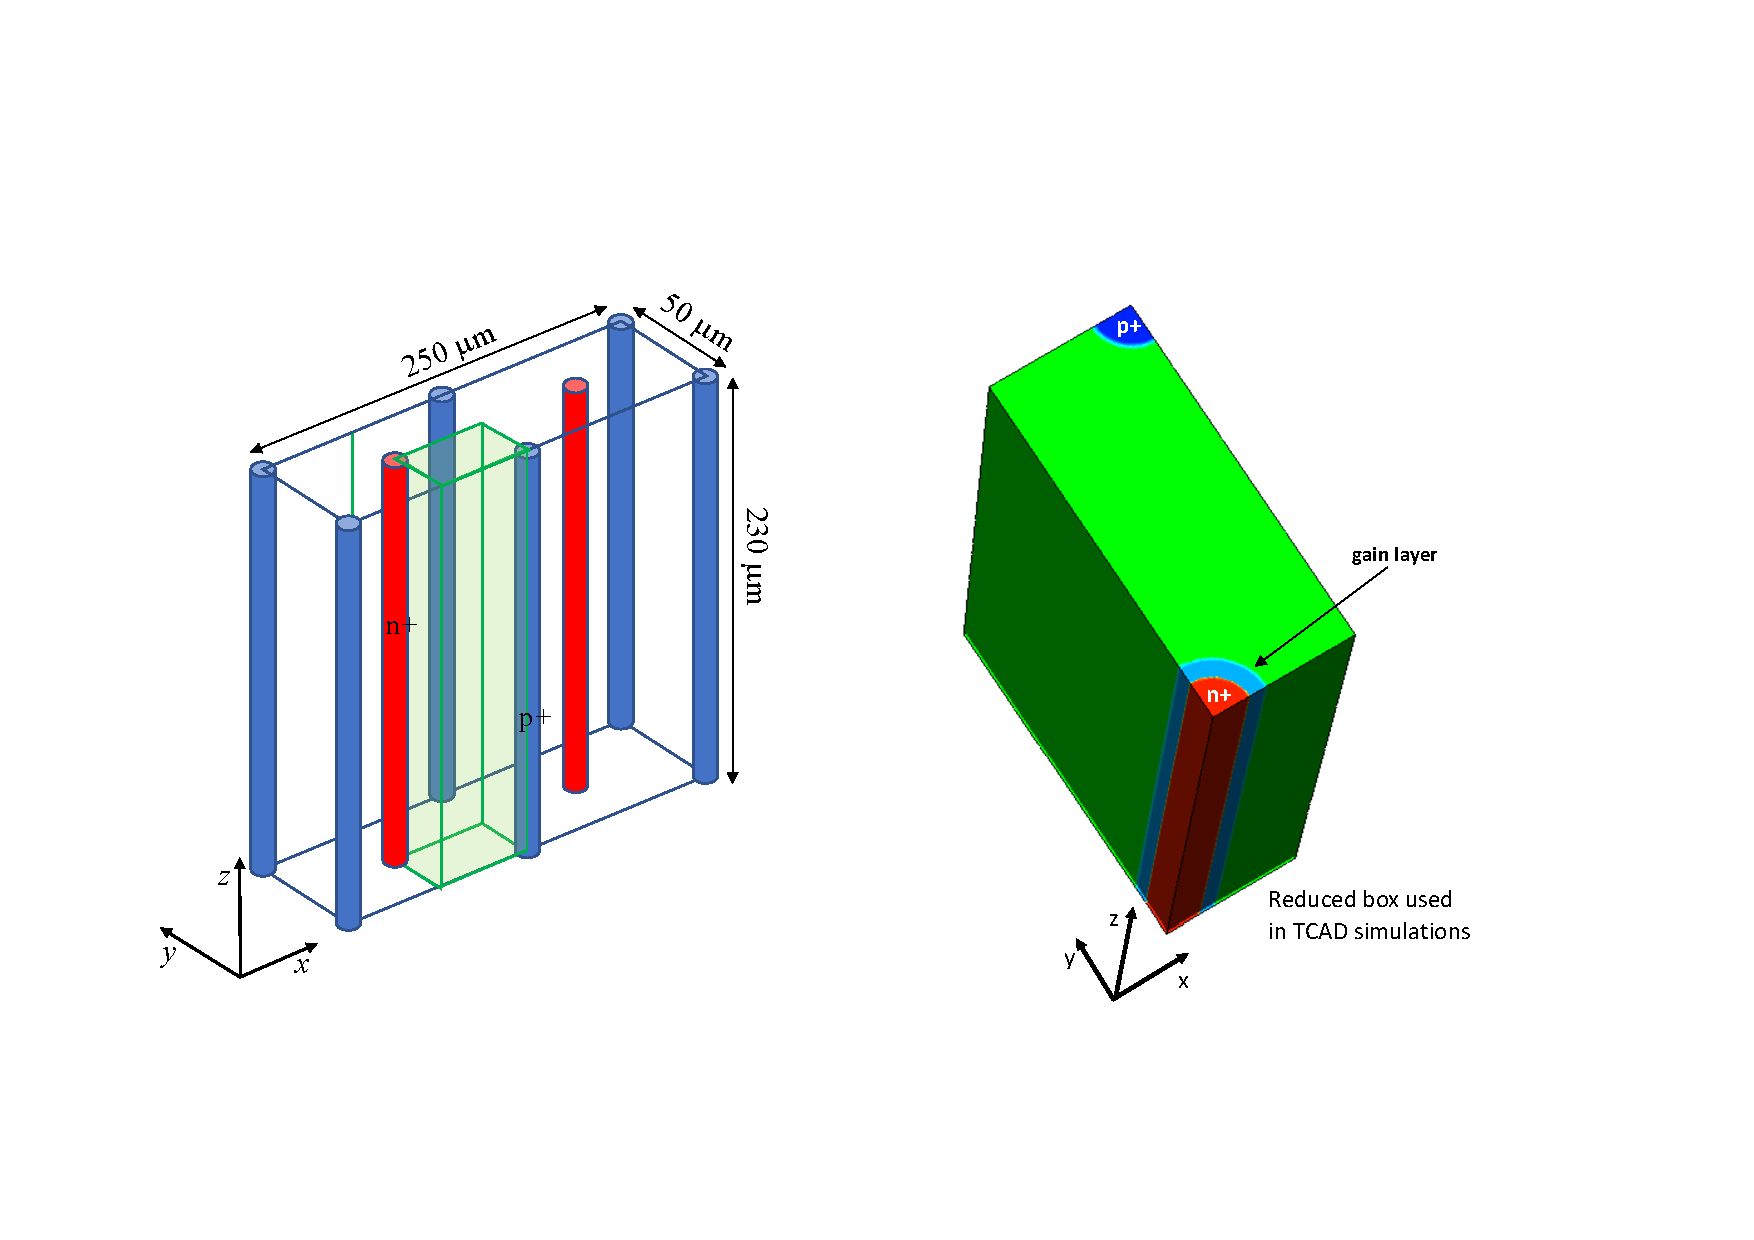
\includegraphics[width=0.60\textwidth,keepaspectratio]{figures1/IBL3D_GL.pdf}
\caption{A schematic view of IBL 3D pixel sensor (left) and the reduced box used in TCAD simulations 
(right).\label{fig:ibl-3d}}
\end{center}
\end{figure}

\section{LGAD}

The planar LGAD detector has a gain layer that contains high electric field to
cause multiplication of charge carries that transverse the region.
The gain is achieved by raising the electric field high enough to enable the
charge carriers to create secondary ionization during the charge collection process.
The main difference to standard APD detectors are the low gain
required to detect high energy charged particles in the thin sensors.
With the low gain these sensors can be very thin to have a fast drift time
and have enough signal-to-noise ratio to achieve good time resolution.

The fast timing detector has been studied extensively for HL-LHC upgrades where the
excellent time resolution coupled with good spatial resolution can help to
reduce pile-up events. ATLAS has recently proposed to use the High Granularity
Timing Detector (HGTD) in the forward region and CMS is considering adding
a timing layer in the barrel region with SIPM for photon detection, while using HGTD
in the forward region. In both cases, the timing detector is 
limited to have a pad size of 1 mm x 1 mm with a time resolution of $\approx$30~ps, but this 
size is too large to be useful for precision tracking.

\begin{figure}[hbtp]
\begin{center}
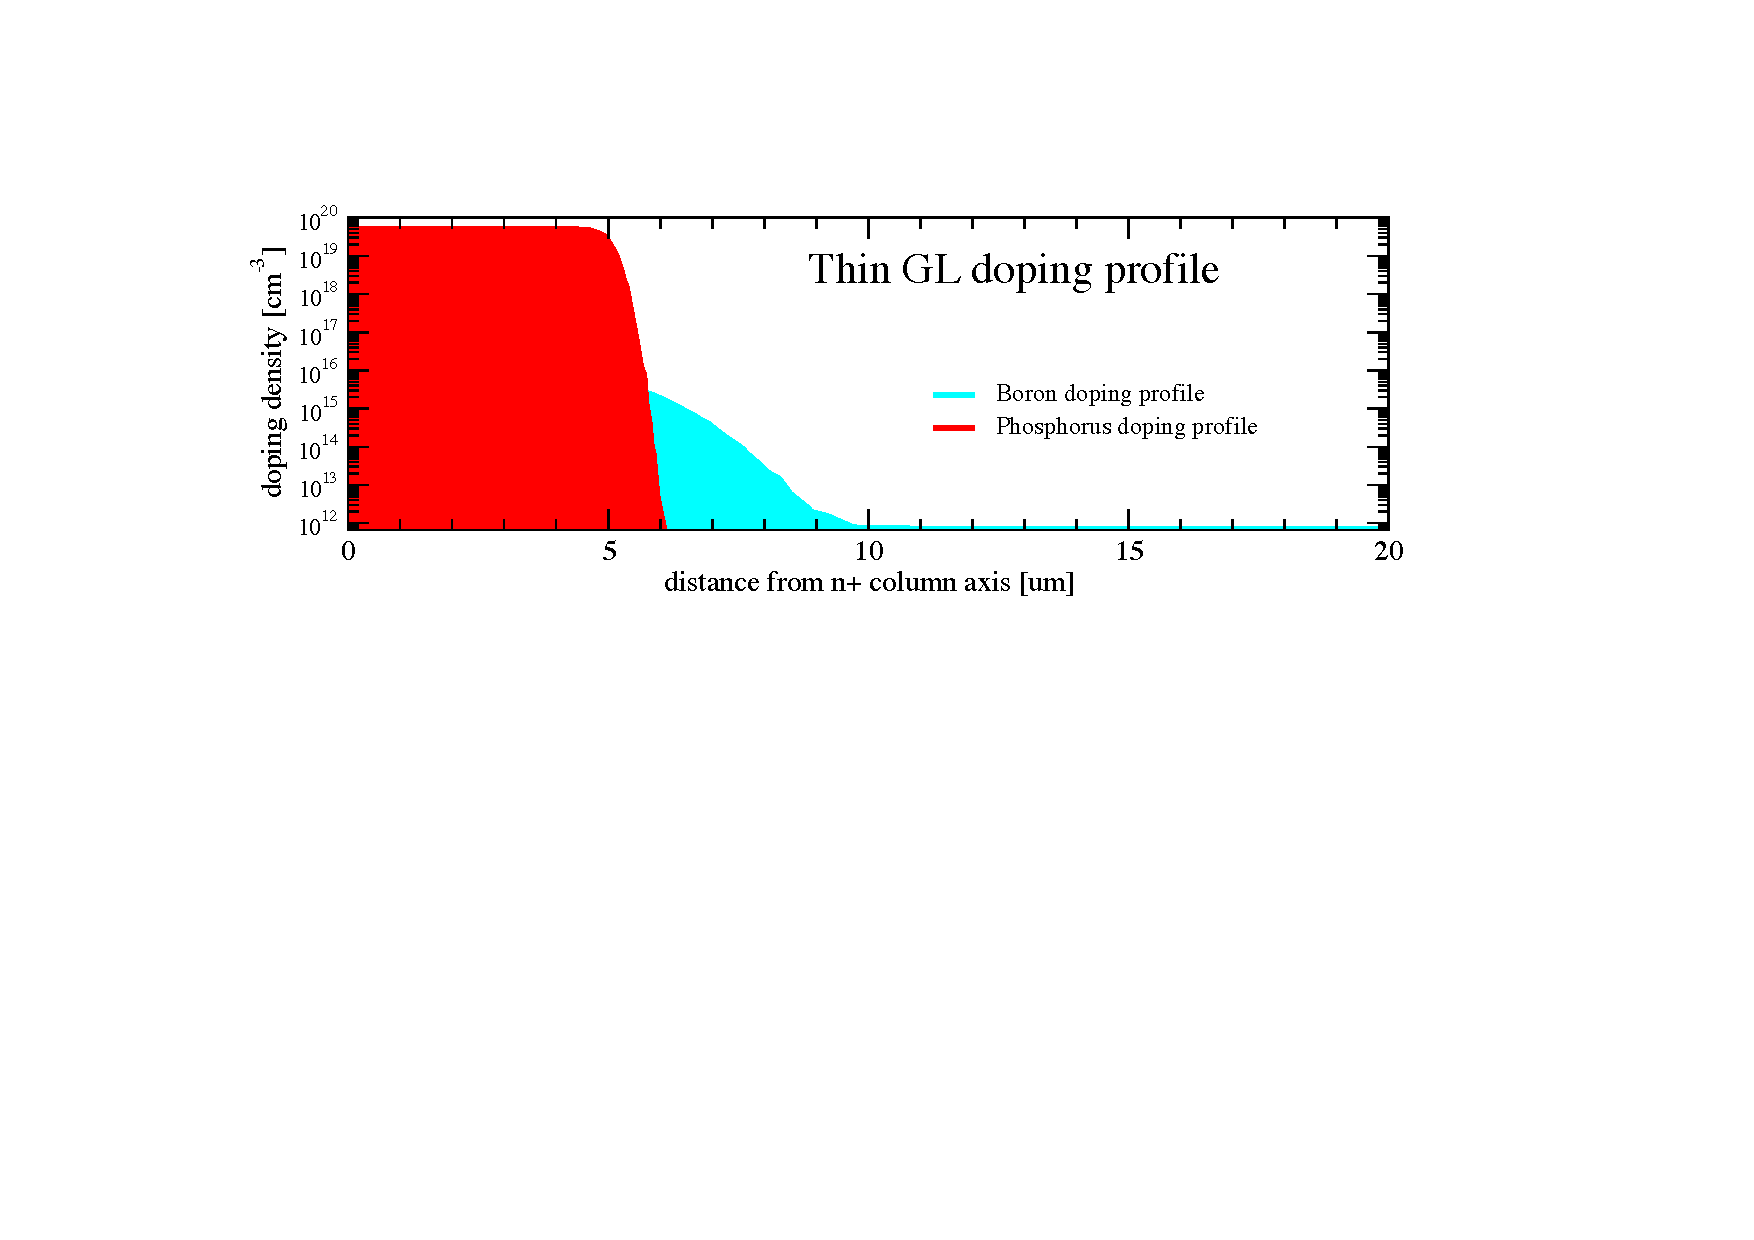
\includegraphics[width=0.49\textwidth,keepaspectratio]{figures1/ThinDopingProfile.pdf}
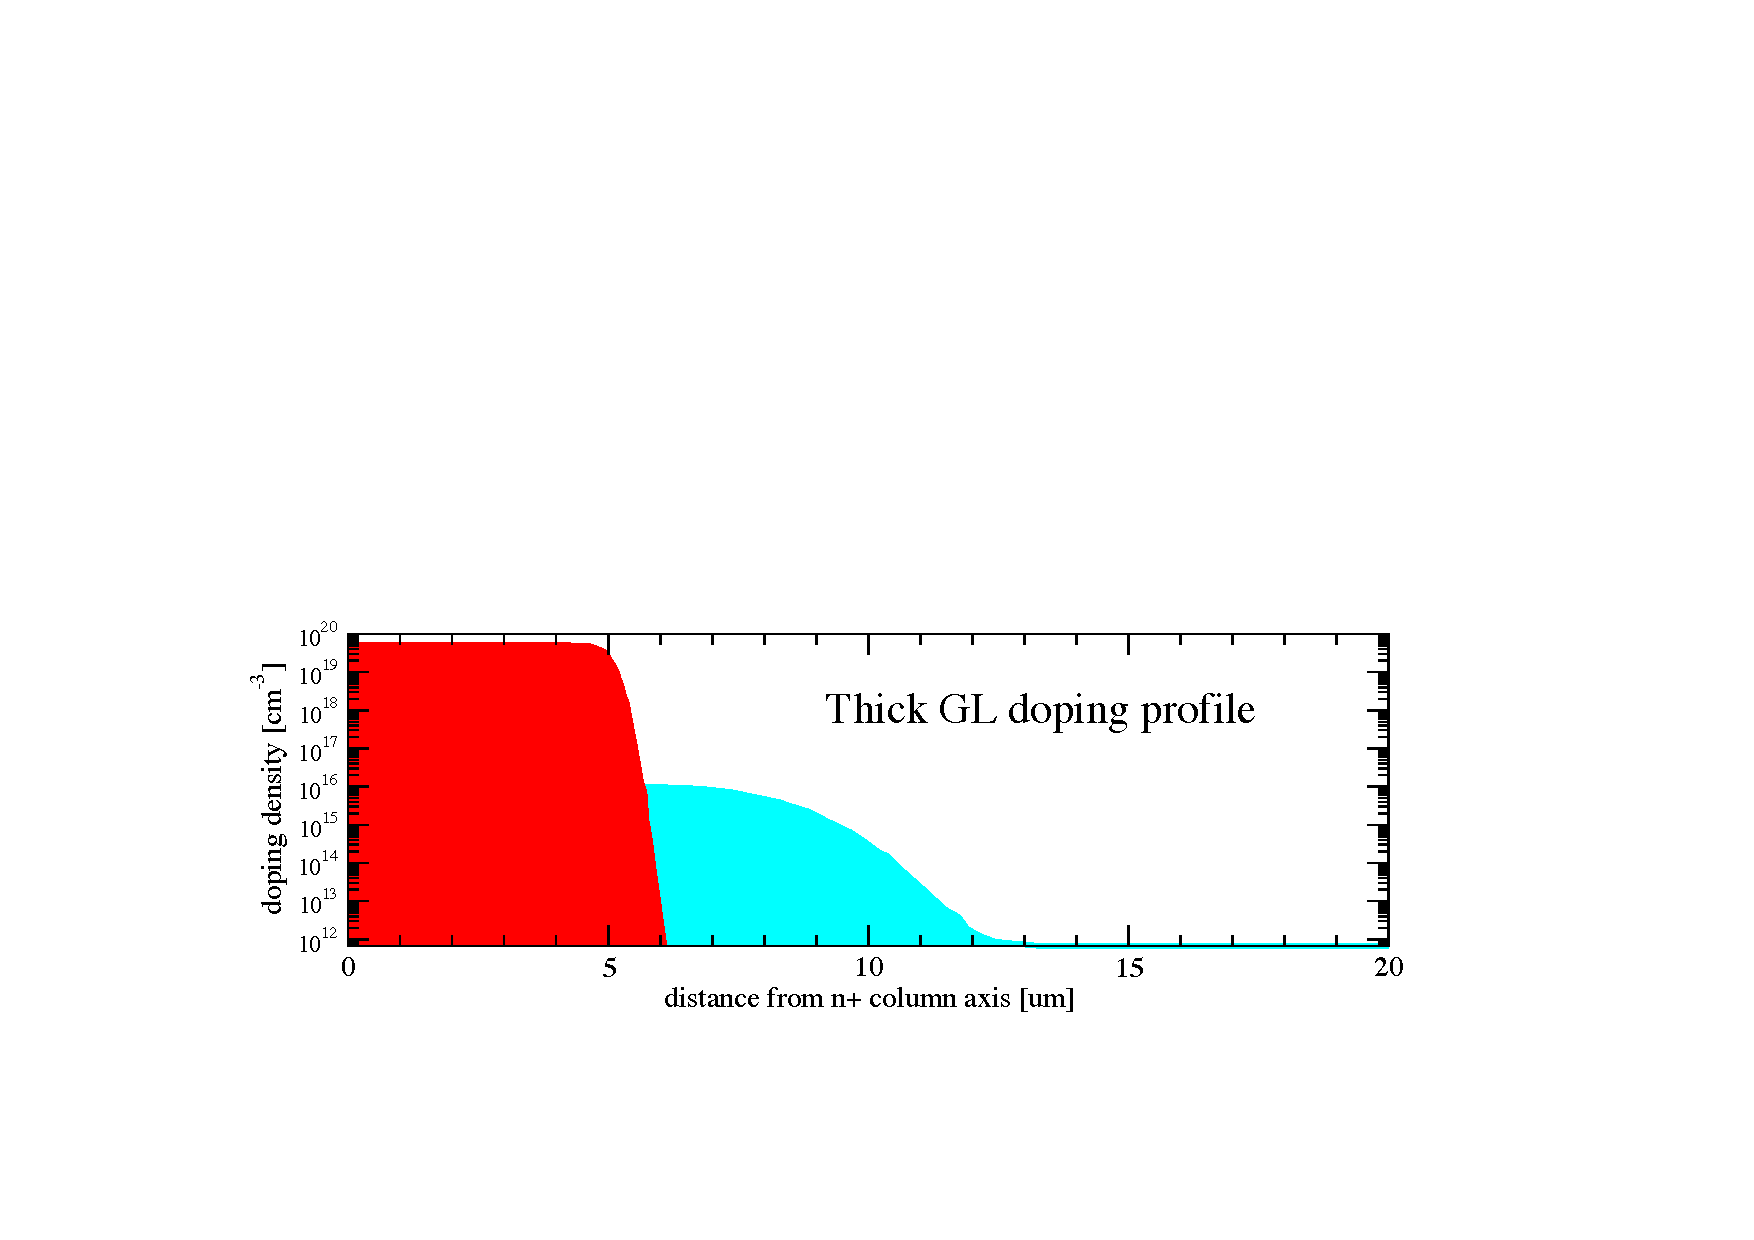
\includegraphics[width=0.49\textwidth,keepaspectratio]{figures1/ThickDopingProfile.pdf}
\caption{An example of boron and phosphorous doping concentration profiles for $n+$ readout electrode (in red) and gain layer (light blue), respectively. The phosphorous doping profiles in left and right panels were obtained with short and long diffusion times, respectively; maximum value of phosphorous concentration were changed in the simulations to test the properties of gain layer.\label{fig:DopingProfiles}} 
\end{center}
\end{figure}

The timing resolution is determined mainly by contributions from time walk and noise
jitter. The time walk contribution is usually minimized by using Constant Fraction
Discrimination (CFD) or determining time of the signal crossing fixed threshold.
The jitter contribution is determined by the rise of the signal at the output of
the amplifier and noise level. The timing resolution can be improved with larger
gain as well as with thin detectors since both increase the slew-rate of the amplifiers.
However, the time walk is dominated by Landau fluctuations due to
the non-uniform charge deposition within the sensors, especially for LGADs where
electrons need to reach the gain layer to multiply

\begin{figure}[hbtp]
\begin{center}
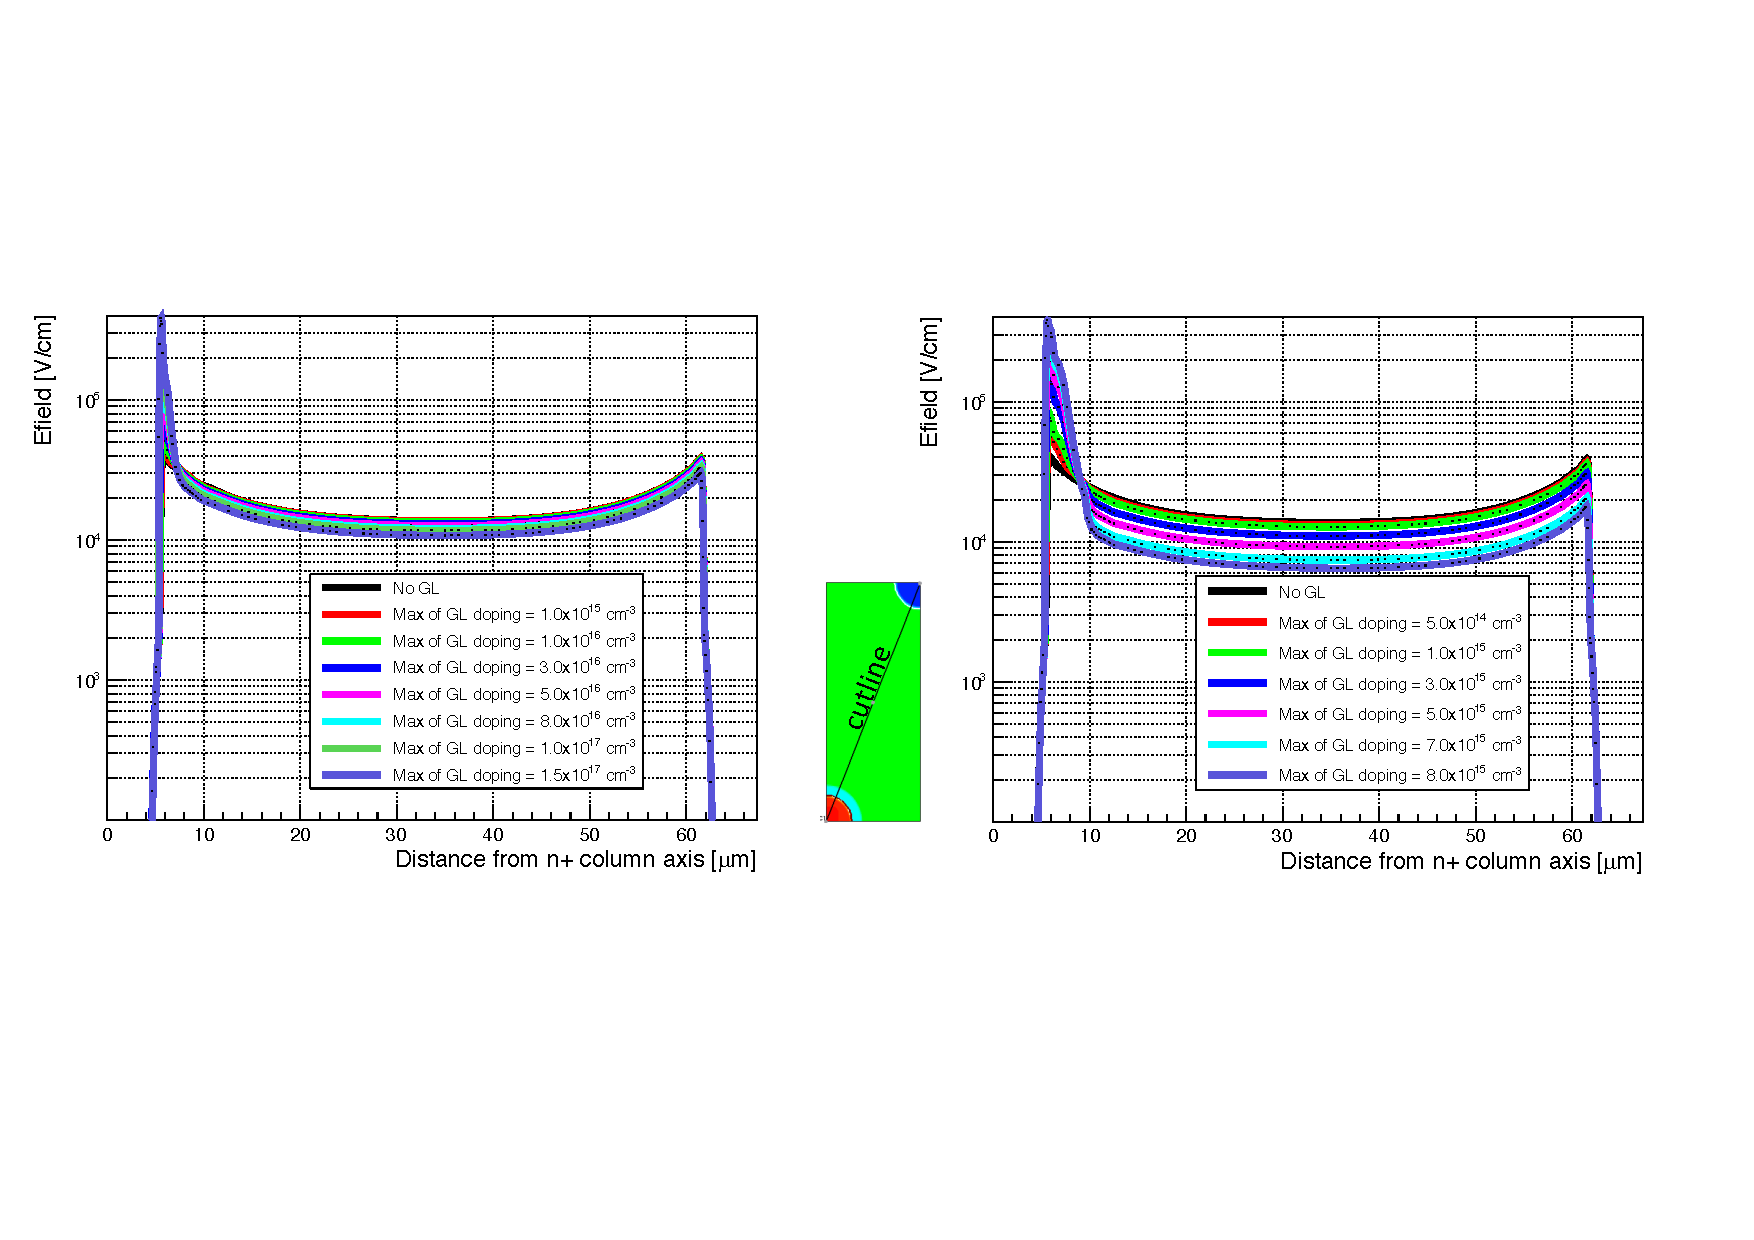
\includegraphics[width=0.80\textwidth,keepaspectratio]{figures1/ThinThickEfield.pdf}
\caption{Electric field values along the diagonal line between n+ and p+ electrodes with a bias voltage of 100V for thin (left) and thick (right) doping profiles. Note the increase of the high electric field region for the thick GL.\label{fig:efield}} 
\end{center}
\end{figure}

\section{TCAD simulation}
The simulation is performed using the Synopsys Sentaurus TCAD simulation toolkit
to understand the electrical behavior for the proposed 3D-LGAD sensor. 
We use the same TCAD setup for the ATLAS IBL 3D pixel detector study and
simply add an extra thin low-resistivity p+ doping gain layer of $3\div 4\ \mu$ thick
surrounding the n+ readout electrode. The IBL 3D pixel cell consists of two connected n+ 
readout electrodes (2E) surrounded by eight p+ electrodes with a size of 50x250x230 $\mu m^3$
as shown in Fig.~\ref{fig:ibl-3d}. By taking the advantage of 8--fold symmetry of IBL 3D pixel and to save time, TCAD simulations were done in the reduced green box shown in Fig.~\ref{fig:ibl-3d}. 

\subsection{Gain Layer doping profiles}

As mentioned in section II, the gain layer were obtained by adding a thin ($3\div 4$ $\mu m$ of thickness) low--resitivity diffusion layer doped with phosphorus. We have considered different gain layer doping profiles by changing both the maximum phosphorous concentration and layer thickness (see the examples in  Fig.~\ref{fig:DopingProfiles}); the corresponding electric and charge collection properties have been calculated in many of these situations.

\begin{figure}[h!]
\begin{center}
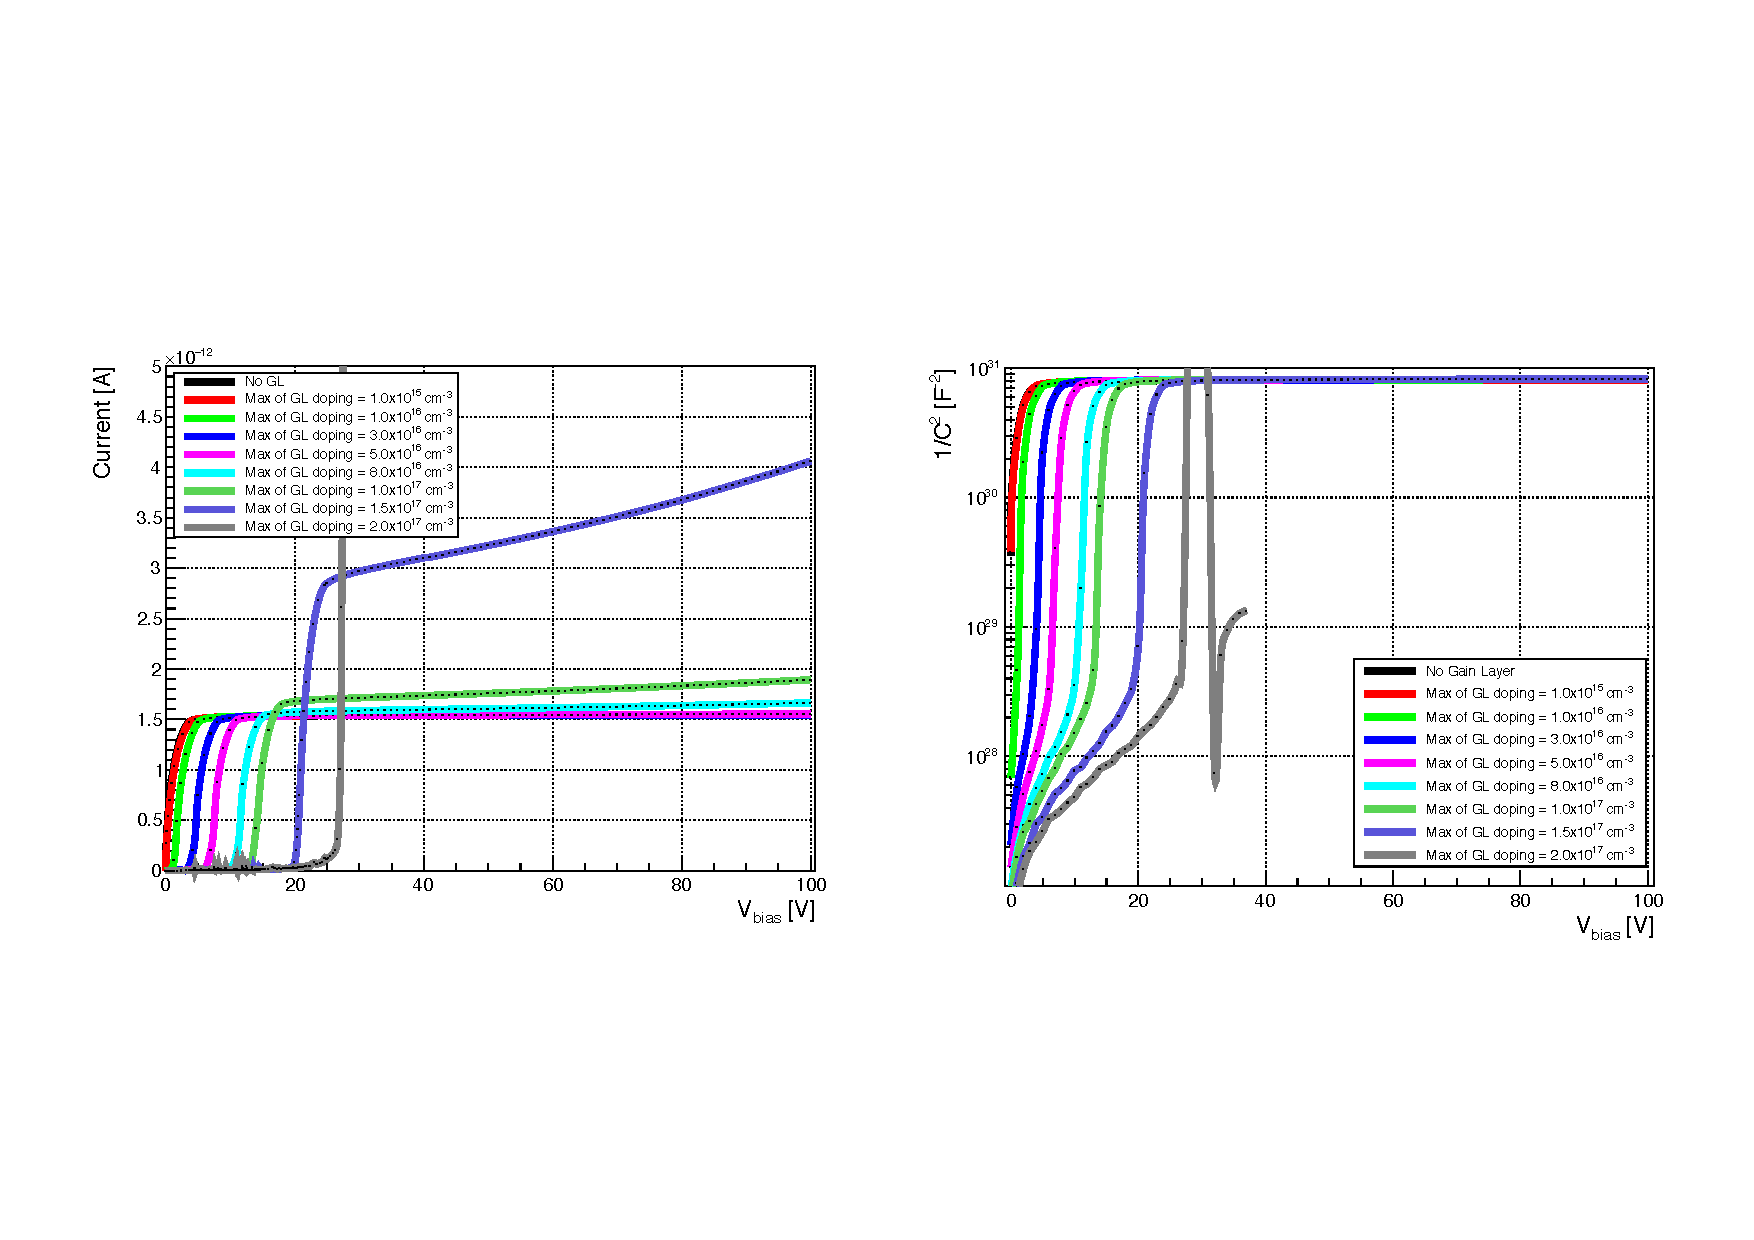
\includegraphics[width=0.80\textwidth,keepaspectratio]{figures1/Thin_IV_CV_curves.pdf}
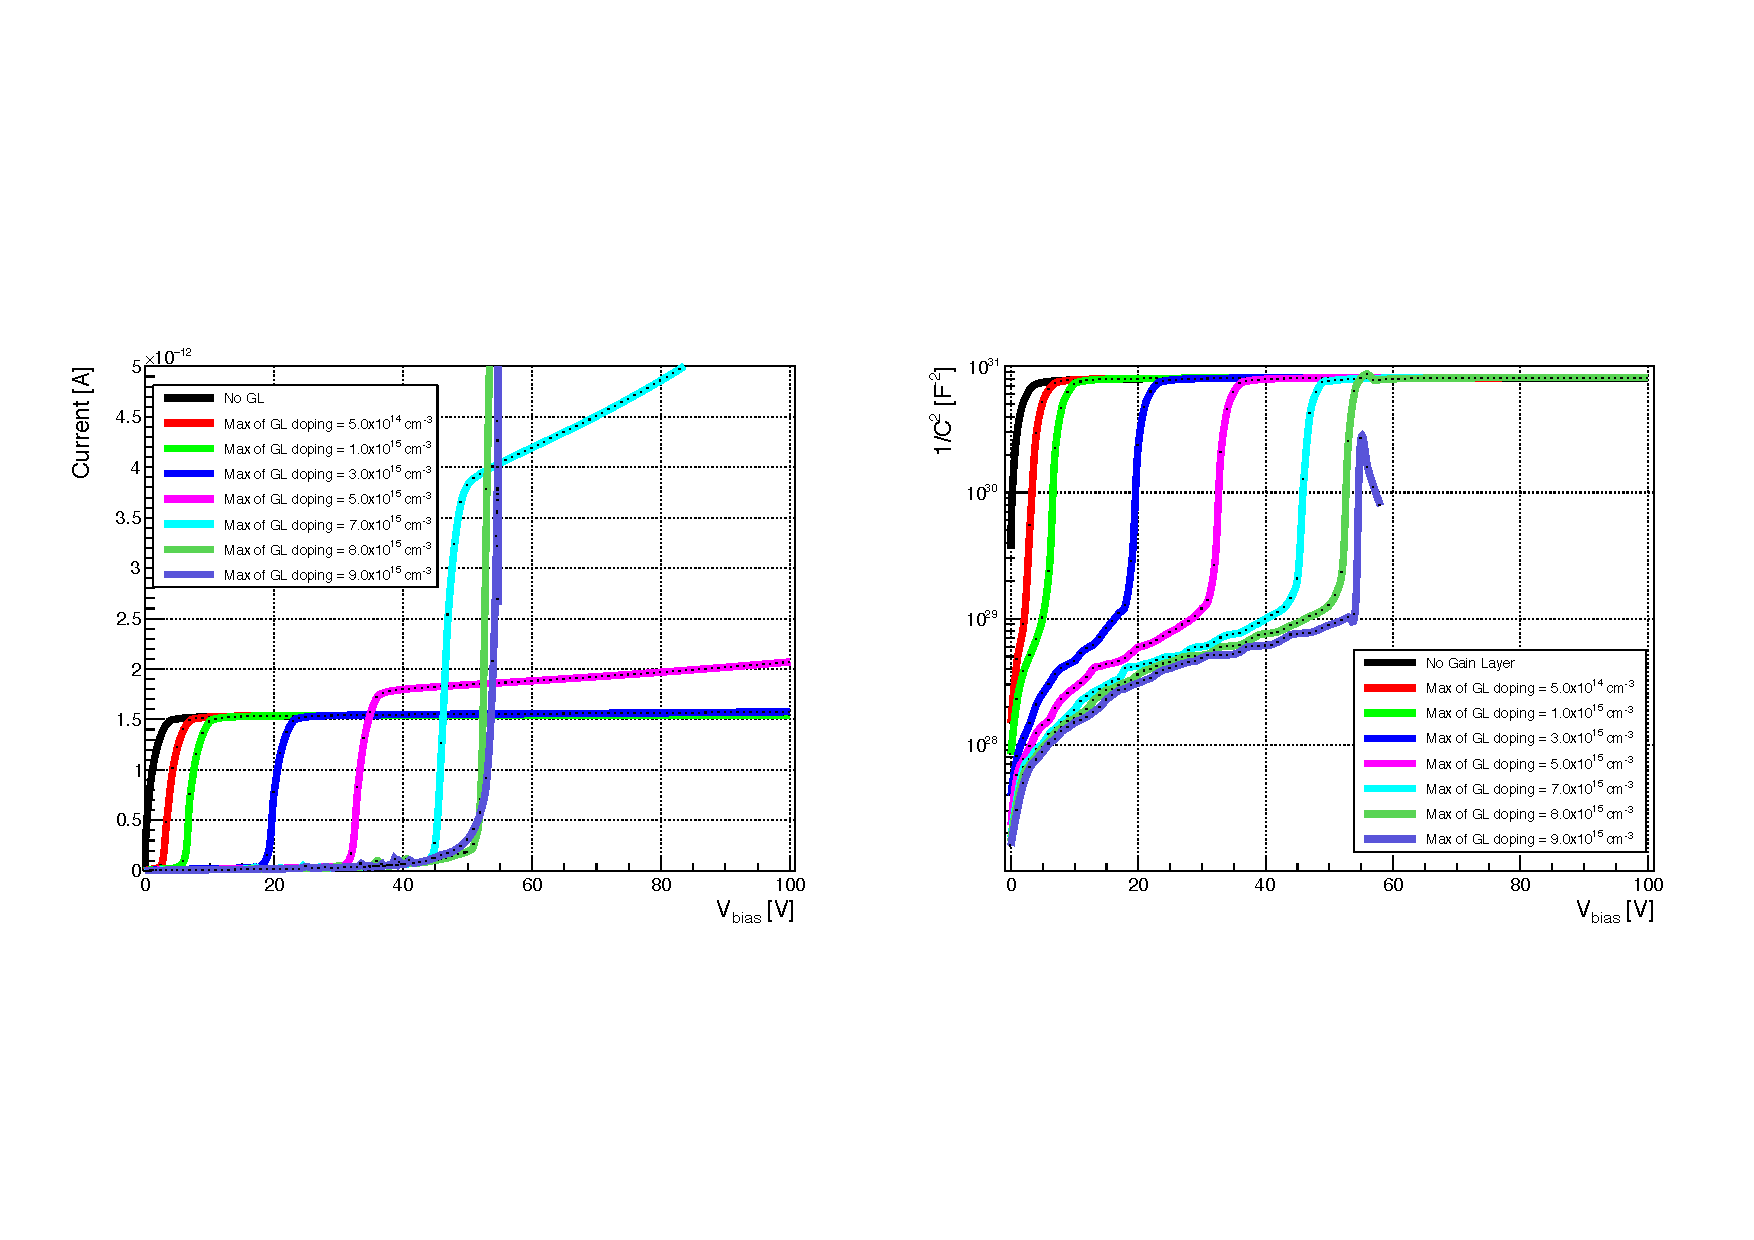
\includegraphics[width=0.80\textwidth,keepaspectratio]{figures1/Thick_IV_CV_curves.pdf}
\end{center}
\caption{The curves for I-V (left panels) and 1/C$^2$-V (right panels) for  thin (top) and thick (bottom) GL profiles  with different maximal doping densities. Note that the low values of the currents in the left panels and the higher values of $1/C^2$ are due to the fact that they correspond those obtained for the reduced box used for the TCAD simulations; for comparison to a practical measure they should be rescaled by taking into account the number of the sensors in a module.
\label{fig:IV-CV}}
\end{figure}

\subsection{Electric properties}    
We have considered different values for the p+ doping concentration of the gain layer (ranging from $10^{14}$ to $1.5\cdot 10^{17}$ cm$^{-3}$). Actually, the highest GL doping value considered for each GL profile is related to the profile thickness; at higher doping concentrations, breakdown takes place before the depletion. For example, for thin and thick GL profiles shown in Fig.~\ref{fig:DopingProfiles}, the corresponding higher p+ doping  concentrations are $1.5\cdot 10^{17}\ \mathrm{cm^{-3}}$ and $8.0\cdot 10^{15}\ \mathrm{cm^{-3}}$, respectively. 

Fig.~\ref{fig:efield} shows the electric field profile along the diagonal line between n+ and p+ electrodes with a bias voltage of 100 V for the unirradiated sensor for thin and thick GL profiles of Fig.~\ref{fig:DopingProfiles}. Note that, as the gain layer doping is increased, the electric field shows the expected increase in the GL region. Note also that for the thick GL profiles (Fig. \ref{fig:efield}, right panel), the same GL high field values are obtained in a wider region and, moreover, for a much lower p+ doping concentration. 



The current-voltage (I-V) curves and the capacitance-voltage (1/C$^2$-V) curves have been also checked for 
different doping densities of the gain layer (GL). As we can see, both for thin and thick gain layer profiles (Fig.~\ref{fig:IV-CV}, upper and lower panels, respectively), there is a perfect correspondence between the jumps in the I-V curves and the jumps in 1/C$^2$ - V curves; this is a clear signature of depletion. Note also how GL increasing doping concentration shifts depletion to higher bias voltages.   

\begin{figure}[hbtp]
\begin{center}
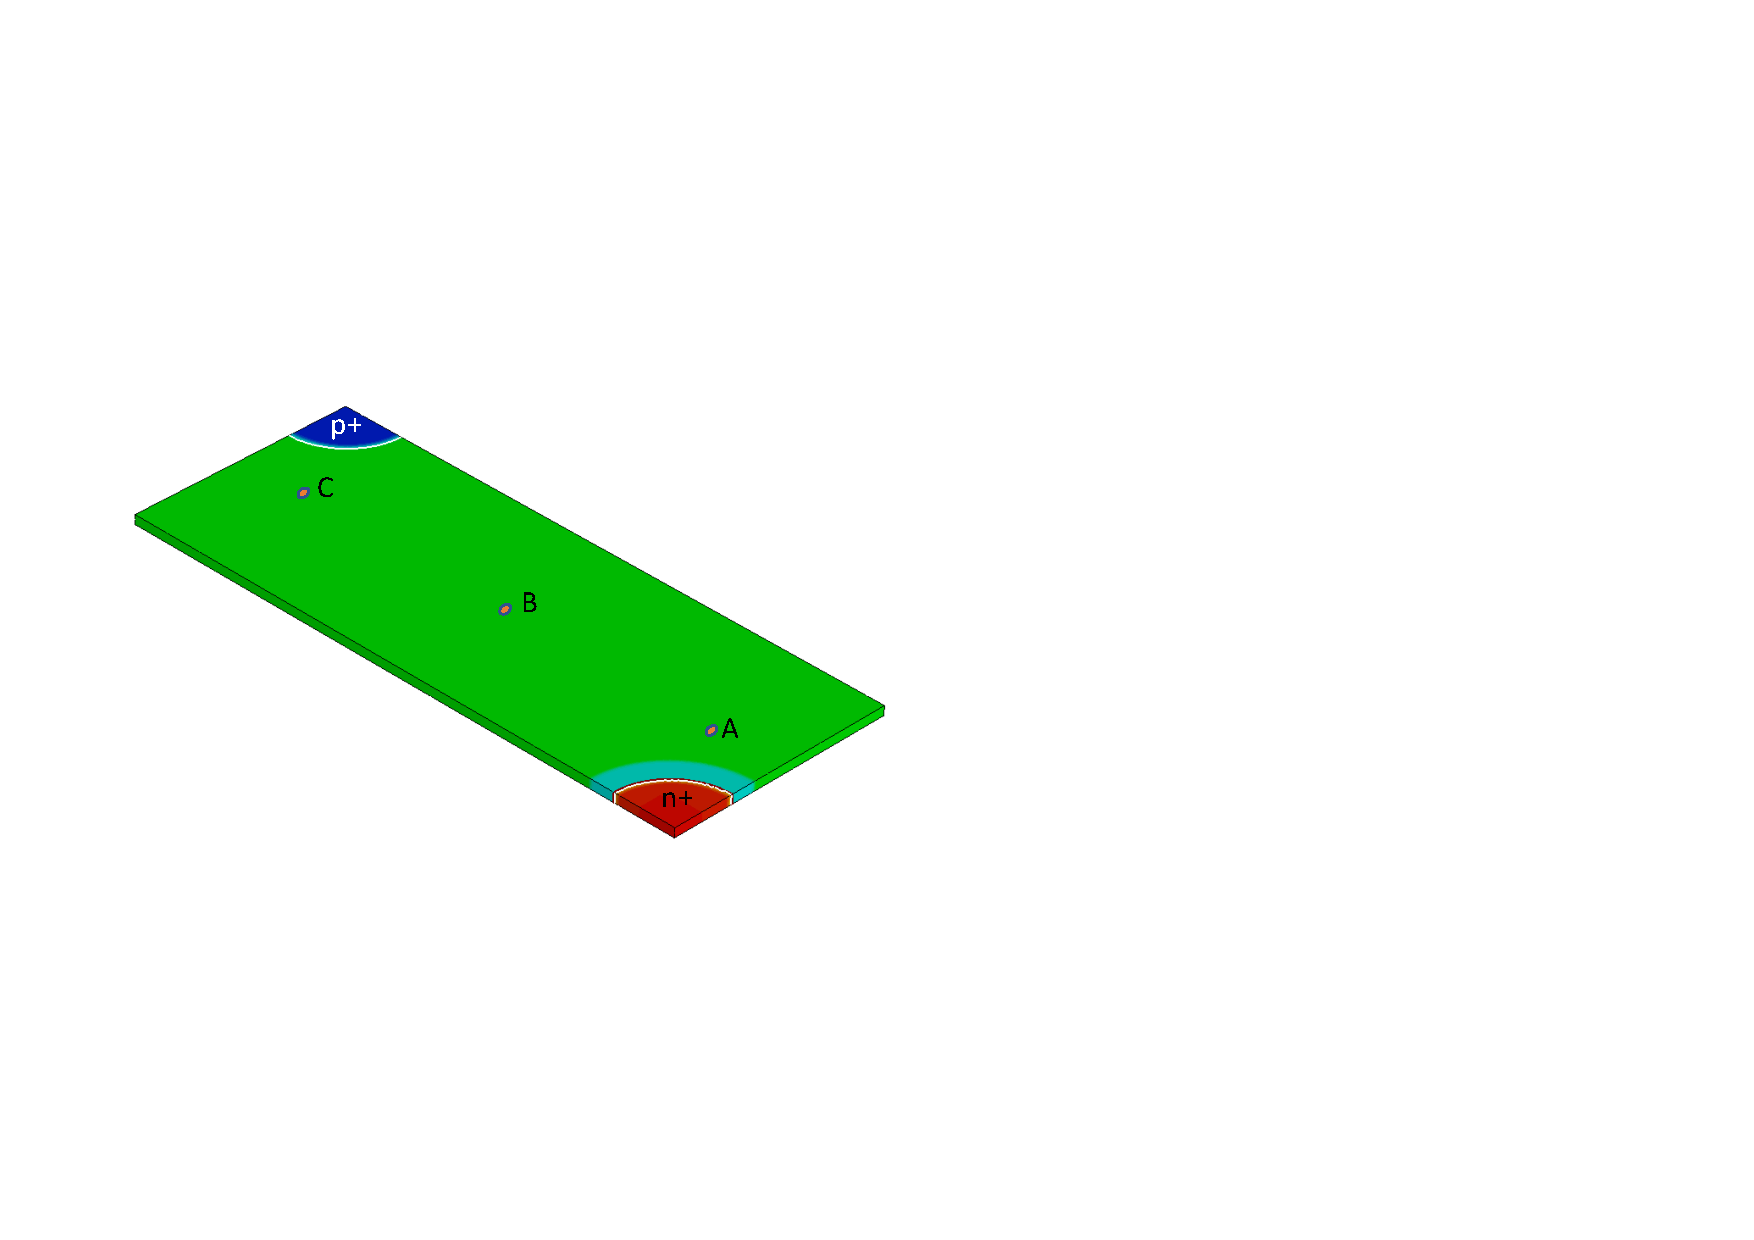
\includegraphics[width=0.4\textwidth,keepaspectratio]{figures1/Slice.pdf}
\caption{The sketch of the reduced sensor area with different positions marked for the MIP passing through perpendicularly in TCAD simulation.\label{fig:box_points}}
\end{center}
\end{figure}

Thin and thick GL profiles show rather different electric properties. In particular, from what shown above, it is evident that, with respect to thin GL profiles, thick profiles have the advantage that, by using a lower doping concentration, the same high electric field values at the GL are reached, but in a wider region. As concerning the sensor properties we are looking for, the larger is the high--field region, the greater is the probability of charge multiplication; this fact led us to choose this configuration as the best candidate for a 3D Low-Gain Avalanche diode. Because of this choice, in the following we will concentrate to the charge collection properties for only 3D diode with thick GL profile.

\begin{figure}[hbtp]
\begin{center}
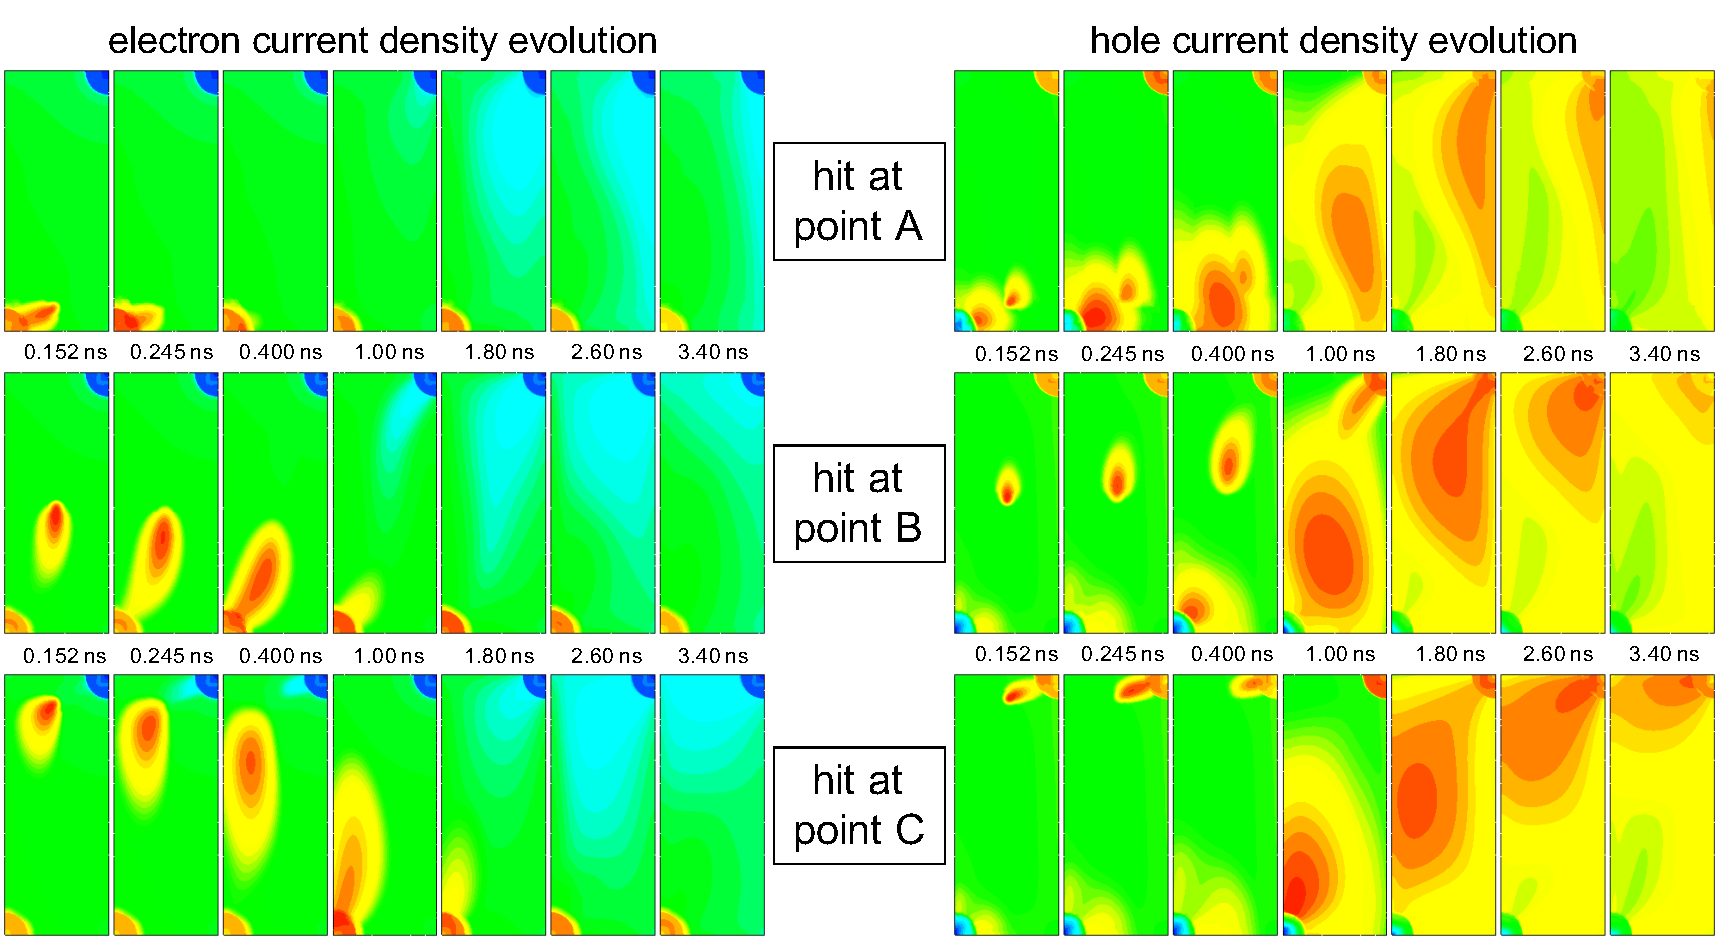
\includegraphics[width=0.80\textwidth,keepaspectratio]{figures1/MIP_current_evolution_ABC.pdf}\hspace{0.7cm}
\caption{Time evolution of the electron (left panels) and hole (rigth panels) current densities after MIP hits at points A (upper panels), B (middle panels) and C (lower panels) as obtained from TCAD simulations. The calculation was done for GL thick doping profile with a $8.0\cdot 10^{15}$ cm$^{-3}$ p+ doping maximum concentration and a bias voltage of $100$ V.\label{fig:MIP-timeevolution}}  
\end{center}
\end{figure}



\subsection{Charge collection and timing resolution} 

A Minimum Ionizing Particle (MIP) is simulated for charge collection using the TCAD simulation. Fig.~\ref{fig:box_points} shows the sketch of the reduced sensor box used in the simulations. Because of the geometry of the sensor, the reduced thickness of the slice (1 $\mu m$) does not affect sensibly the electric field distribution, but this choice allows for a considerable saving of computing time. We tested that the results obtained in this way are consistent with those coming from the simulations with the full thickness sensor. The three selected hit points, are sufficient to understand the full charge collection and timing behavior of the sensor.    
 
\begin{figure}[hbtp]
\begin{center}
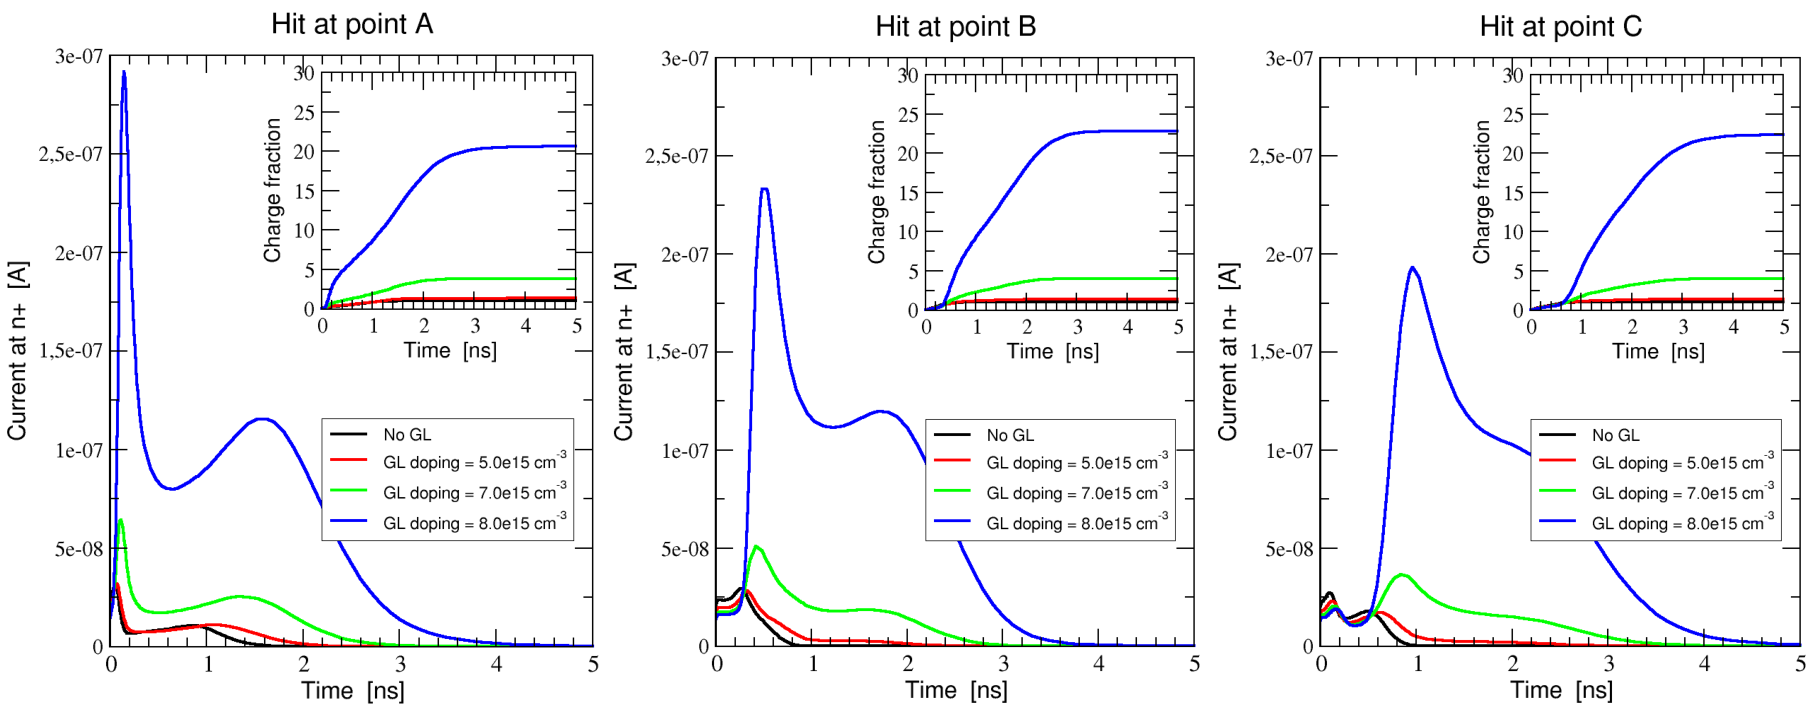
\includegraphics[width=0.95\textwidth,keepaspectratio]{figures1/MIP-ABC-CCE-new.pdf}
\caption{Currents and collected charge fractions as a function of time are shown for hit positions A, B and C, at a bias potential of 100 V and increasing GL doping values.\label{fig:MIP-ABC-CCE-new}}  
\end{center}
\end{figure}

In Fig. \ref{fig:MIP-timeevolution} we can see the time evolution of the electron and hole current densities as obtained by TCAD simulations from MIP perpendicular hits at points A, B and C. The pictures show rather clearly the quick approach of the electrons to the n+ readout electrode and charge multiplication at the GL (surrounding n+) with a consequent production of a slow tail of holes moving toward p+ electrode. Note also the different timing for the three different hit positions.    
 
\begin{figure}[hbtp]
\begin{center}
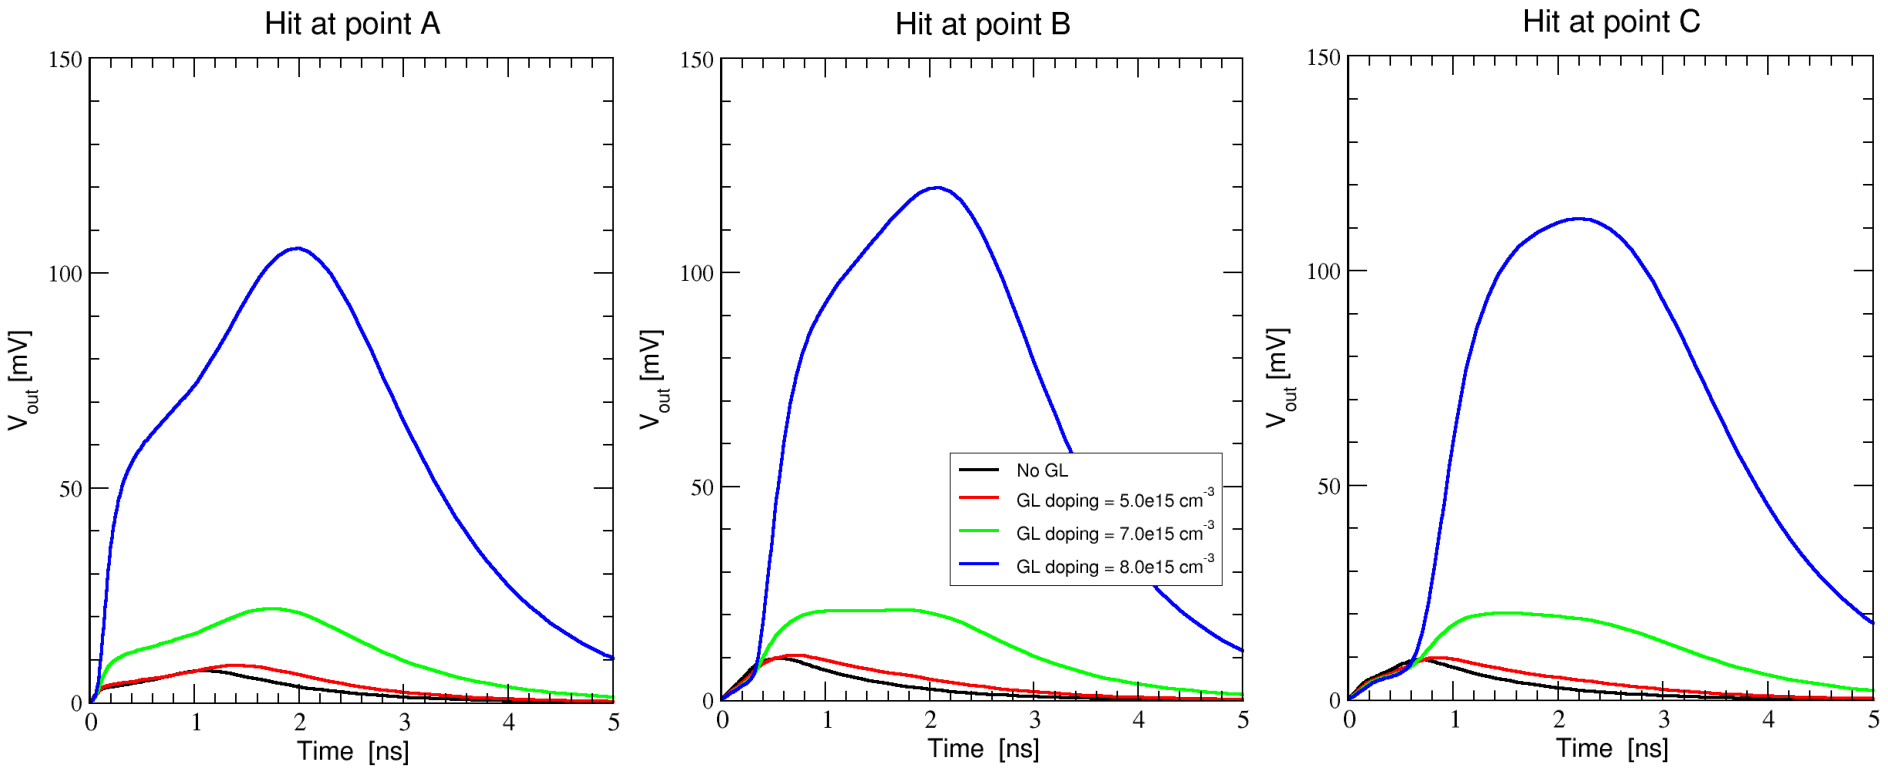
\includegraphics[width=0.90\textwidth,keepaspectratio]{figures1/Shaped_pulses_new.pdf}
\caption{The re--shaped pulses obtained by applying the shaping function mentioned in the text to the current pulses shown in Fig. \ref{fig:MIP-ABC-CCE-new}.\label{fig:Shaped}}
\end{center}
\end{figure}


Fig.~\ref{fig:MIP-ABC-CCE-new} shows some examples for the current and collected charge at the readout electrode for hits at points A, B and C at a bias voltages of 100 V, and for increasing GL doping values. The same scale is used in all graphs, which allows to clearly appreciate the increase in current and collected charge as the GL doping reach high values. A deposited charge by MIP of 80 e (electron charge) per $\mu$m were considered and collected charge is expressed as charge fraction with respect to the deposited one. In our case, since the sensor thickness is 1 um, a charge fraction of 1 means a collected charge = 80 e. Note how collected charge
for GL doping near $8.0\cdot 10^{15}\ \mathrm{cm^{-3}}$ becomes, because of avalanches, also larger than 20 times the deposited charge. Note also that the final collected charge is essentially independent from hit position. 

\begin{table}[hbtp]
\begin{center}
\vspace{-0.5cm}
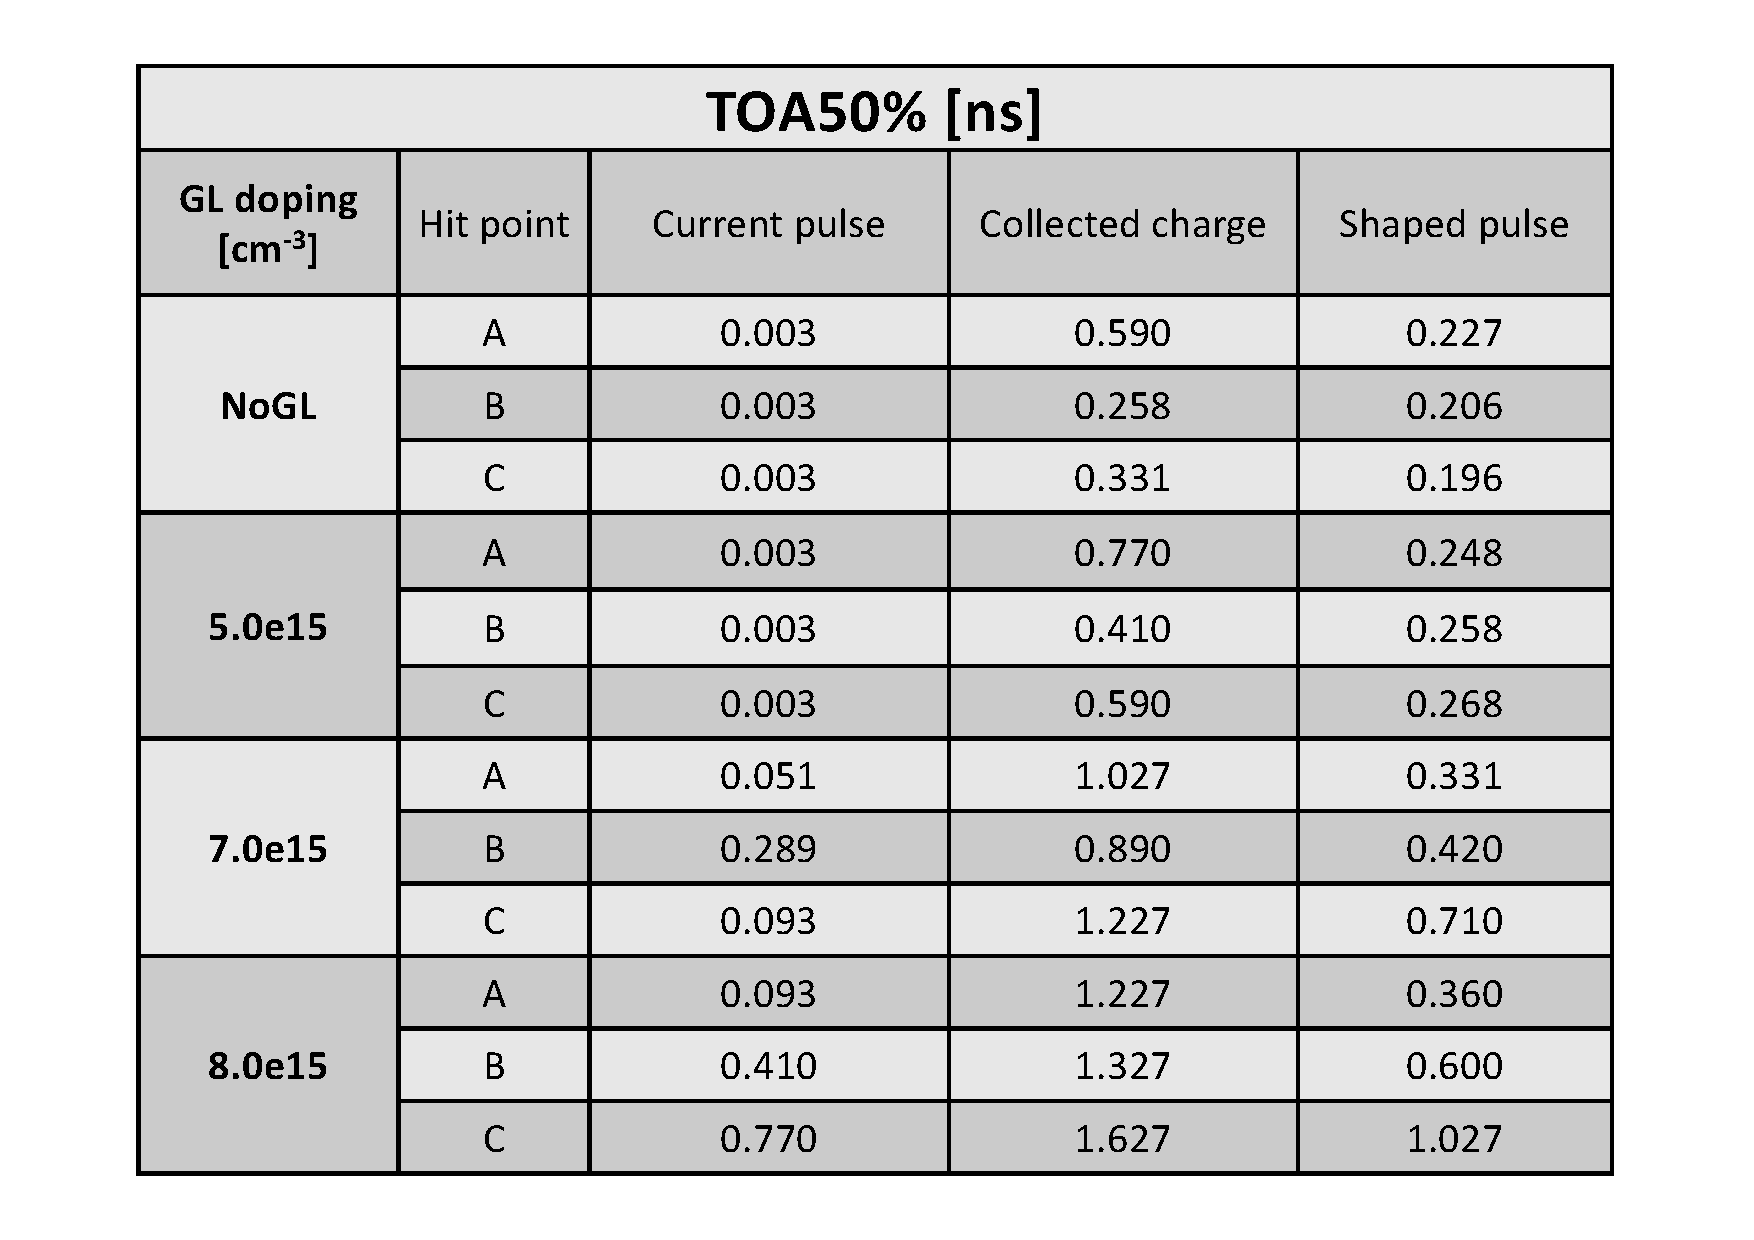
\includegraphics[width=0.6\textwidth,keepaspectratio]{figures1/Table_toa50.pdf}
\caption{The table reasumes the results about the time of arrival at 50\% of the maximal values for current, charge and shaped pulses.\label{Table_times}}
\end{center}
\end{table}
 
Current pulses at the readout electrode is re--shaped by the readout circuits which usually corresponds to an integration process with a function of the following type 
$$
V_{out}(t)=\frac{1}{C_{det}}\mathrm{e}^{-t/\tau_c}\int_0^t i(t^\prime)\mathrm{e}^{t^\prime/\tau_c}dt^\prime
$$
where $C_{det}$ is the detector capacitance. By using this function with $\tau_c=1$ ns, we have re--shaped our pulses obtained by the TCAD simulations. As an example of the re--shaping process, in Fig. \ref{fig:Shaped} we show the re--shaped version of current pulses of Fig.~\ref{fig:MIP-ABC-CCE-new}.

\begin{figure}[hbtp]
\begin{center}
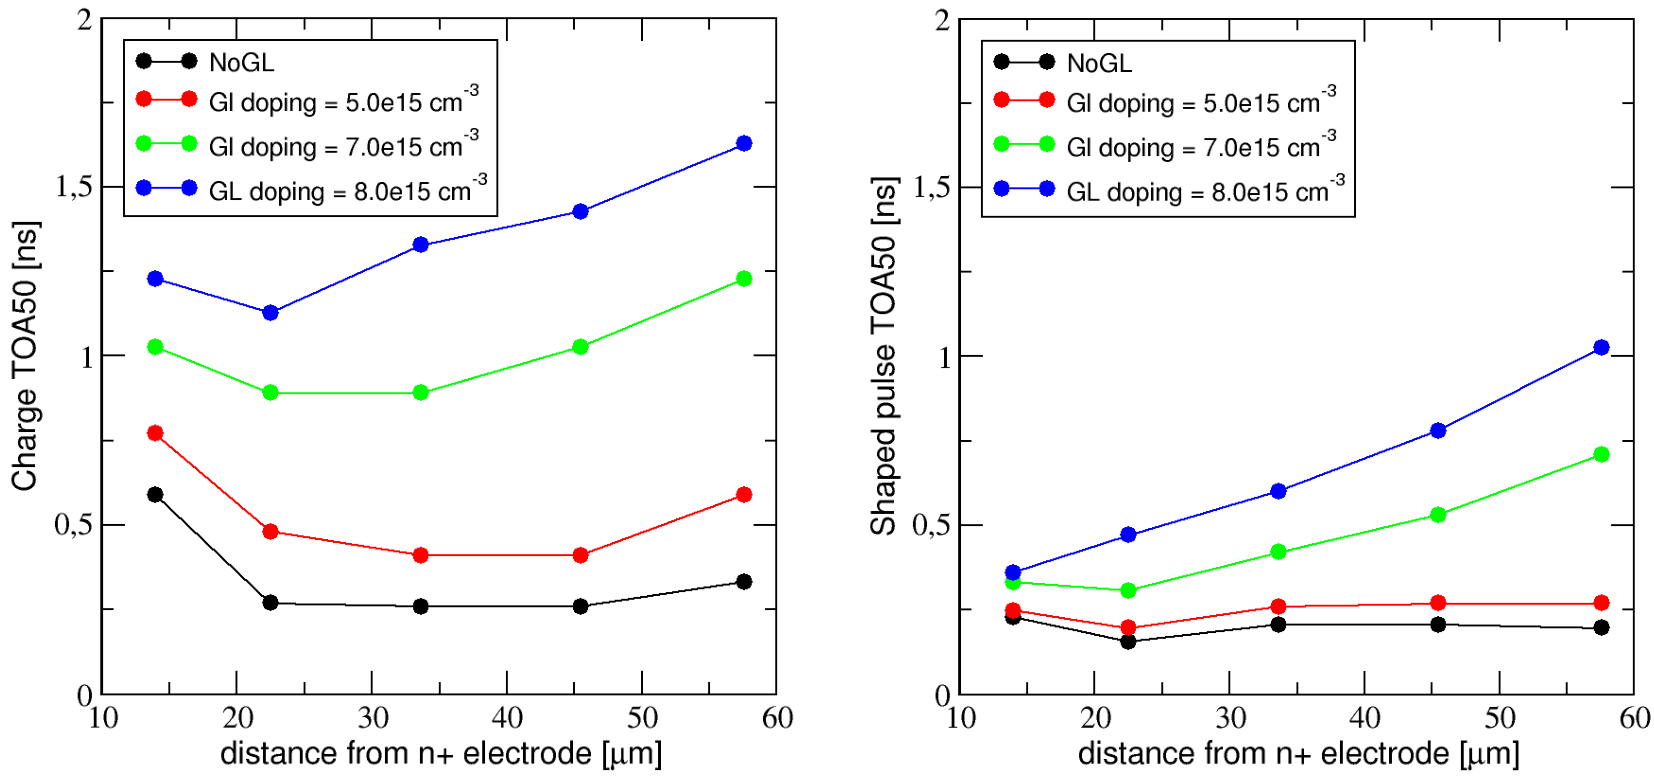
\includegraphics[width=0.74\textwidth,keepaspectratio]{figures1/ToA50_vs_distance.pdf}
\caption{Behavior TOA50 for theposited charge (left panel) and shaped pulse (right panel) as a function of hit distance from the n+ electrode for various GL doping different $V_{bias}=100$ V.~\label{fig:toarms1}}
\end{center}
\end{figure}


The timing of arrival at 50\% of charge pulse height resolution (TOA50) is measured for these hits 
as a function of the distance from the n+ readout electrode in the transverse plane for different bias voltages and the GL doping densities; the results are summarized in Table~\ref{Table_times}. The table shows that TOA50 increases both for increasing distance of the hit point from n+ electrode and for GL doping. This trends are also confirmed by the curves in Fig.~\ref{fig:toarms1} where TOA50 for deposited charge and shaped pulses are plotted versus hit distances (from n+ electrode) for different GL doping concentrations. Such a behavior seems clearly due to the slow drift of the holes produced from the avalanches.  

On the other hand, in Fig. \ref{fig:toarms2} the TOA50 averaged over 5 different distances are plotted as a function of GL doping and confirm that trend.


\begin{figure}[hbtp]
\begin{center}
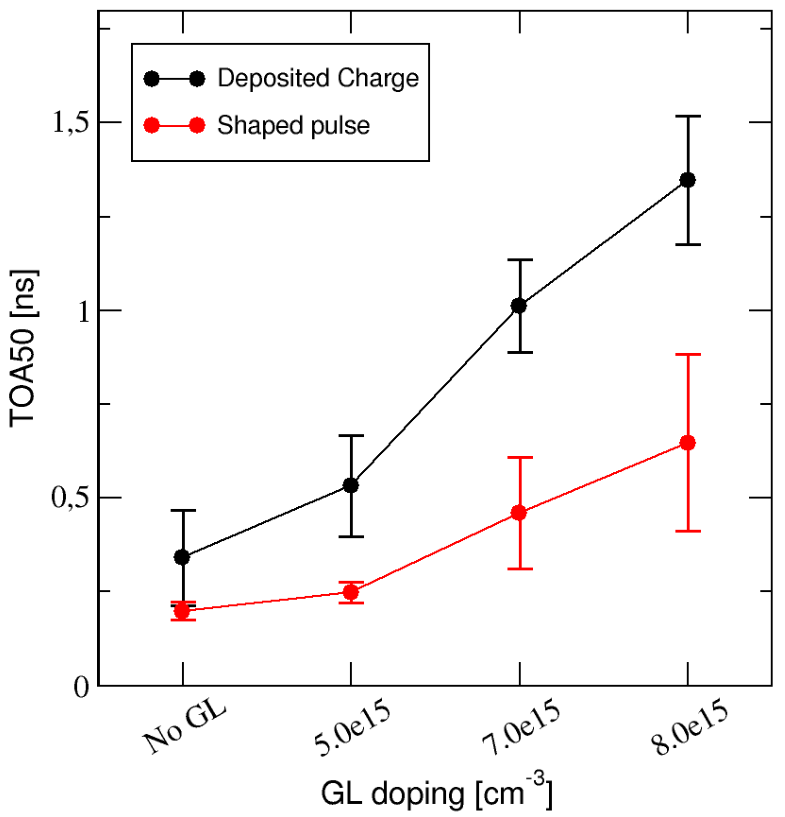
\includegraphics[width=0.40\textwidth,keepaspectratio]{figures1/ToA50_vs_GLdoping.pdf}
\caption{The averages and RMS of 9 measured TOA50 as a function of GL densities and with different bias 
voltages.~\label{fig:toarms2}}
\end{center}
\end{figure}


However, more studies are need to understand better the avalanche process in TCAD simulation and the noise 
level of the front end electronics.   

\section{Monte Carlo Simulations}

In alternative to TCAD simulation, charge collection properties of our prototype sensor have been evaluated also by a Monte Carlo approach. In this approach, making use of the electric field maps of the sensor from TCAD, drift paths of electrons and holes generated by a MIP can be calculated (also including thermal diffusion). 

Charge multiplication process at the GL can be also implemented by importing the electron and hole ionization coefficients e--$\alpha$ and h--$\alpha$ from TCAD simulations. These quantities are strongly amplified at the GL where electric field reaches critical values; so, traveling electrons and holes can create new electron/hole pairs with a probability proportional to the corresponding ionization coefficients times the traveled distance.    

We have verified that the avalanches at the GL can be simulated also with this approach. At the moment, the agreement between the results of this approach and those of the TCAD simulations are not perfect; our Monte Carlo approach gives a deposited charge with is half of that predicted by TCAD simulations. On the other hand, as shown in Fig.~\ref{fig:NewChargeFraction}, the charge time evolution displayed by the two methods are very close each other. 

\begin{figure}[hbtp]
\begin{center}
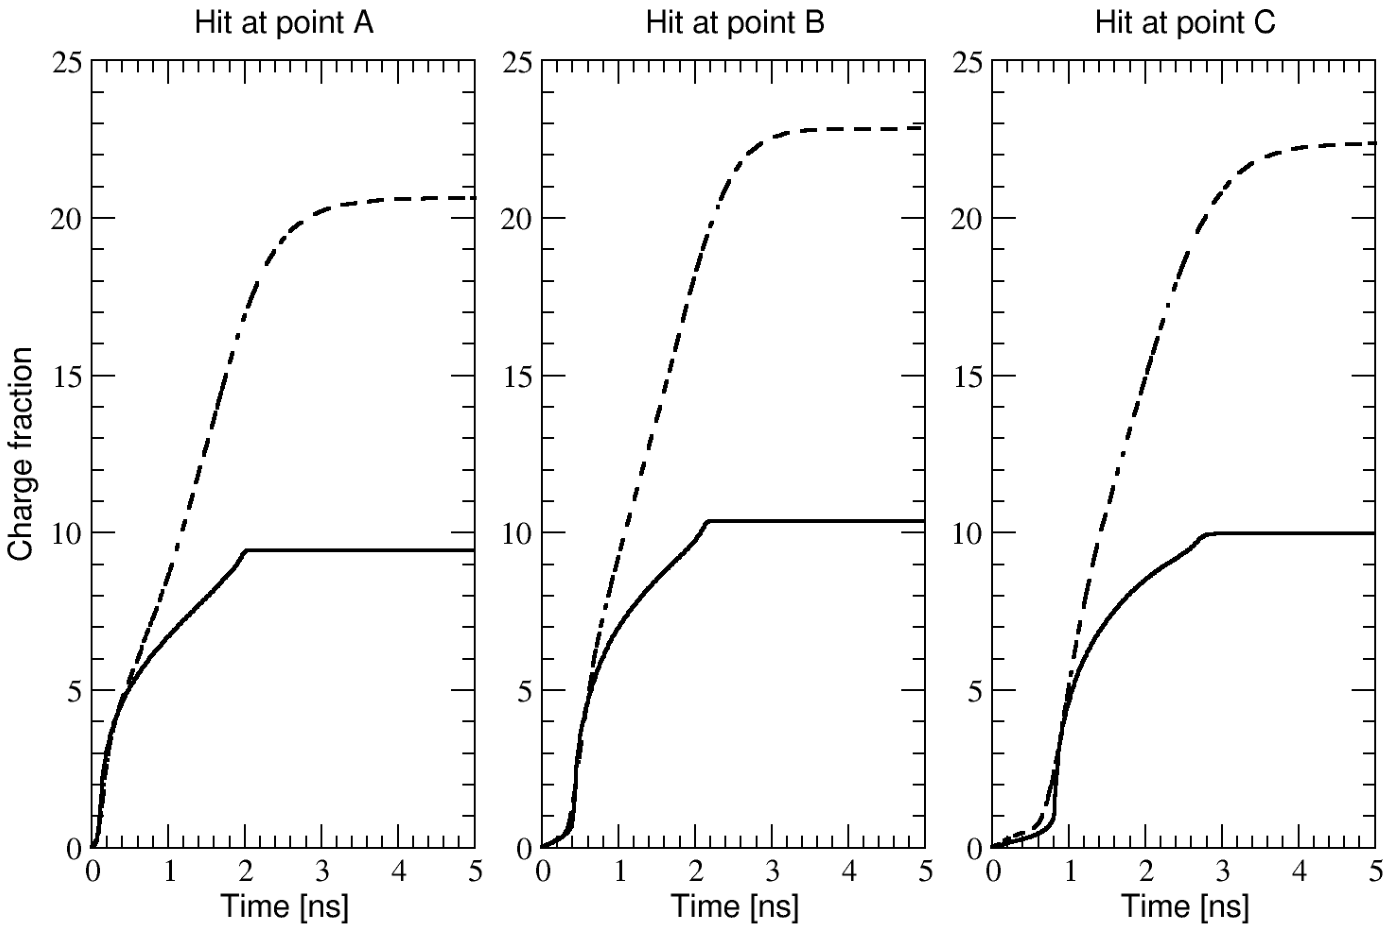
\includegraphics[width=0.8\textwidth,keepaspectratio]{figures1/NewChargeFraction.pdf}
\caption{The collected charge fractions as a function of time as obtained with the Monte Carlo approach are shown (heavy continuos lines) for hit positions A, B and C in the case of a GL doping of $8.0\times 10^{15}\ \mathrm{cm^{-3}}$ and a bias potential of 100 V. Dashed lines correspond to charge fractions obtained in the same conditions with TCAD simulations.\label{fig:NewChargeFraction}}
\end{center}
\end{figure}


\section{Alternative studies with KDetSim} 

We also performed the studies using KDetSim~\cite{kdetsim} to simulate the charge collection in the proposed 3D-GLAD sensor.
The charge drift is simulated in steps with diffusion, impact ionization, and trapping also taken into account and  
the induced current is then proceeded with a transfer function of a front-end electronics with a shaping time of 1 ns. 
The results obtained from KDetSim are consistent with TCAD simulation. Fig.~\ref{fig:kdetgain} shows the projected 
electric fields (V/um) and the average charge collection gains for a MIP passing through randomly and perpendicularly 
to the detector as a function of GL doping densities and the bias voltage. Fig.~\ref{fig:kdettoa} shows the drift-time 
(TOA50) as a function of drift distance from the n+ electrode as well as the average TOA50 before and after the drift-time corrections based on the drift distance. The average TOA50 seems increased for a higher doping density GL, which is mainly 
due to increased the number of holes from the impact ionization process. However, after the drift-distance correction, the 
TOA50 timing resolution can be greatly improved to below 30~ps.  
     
\begin{figure}[hbtp]
\begin{center}
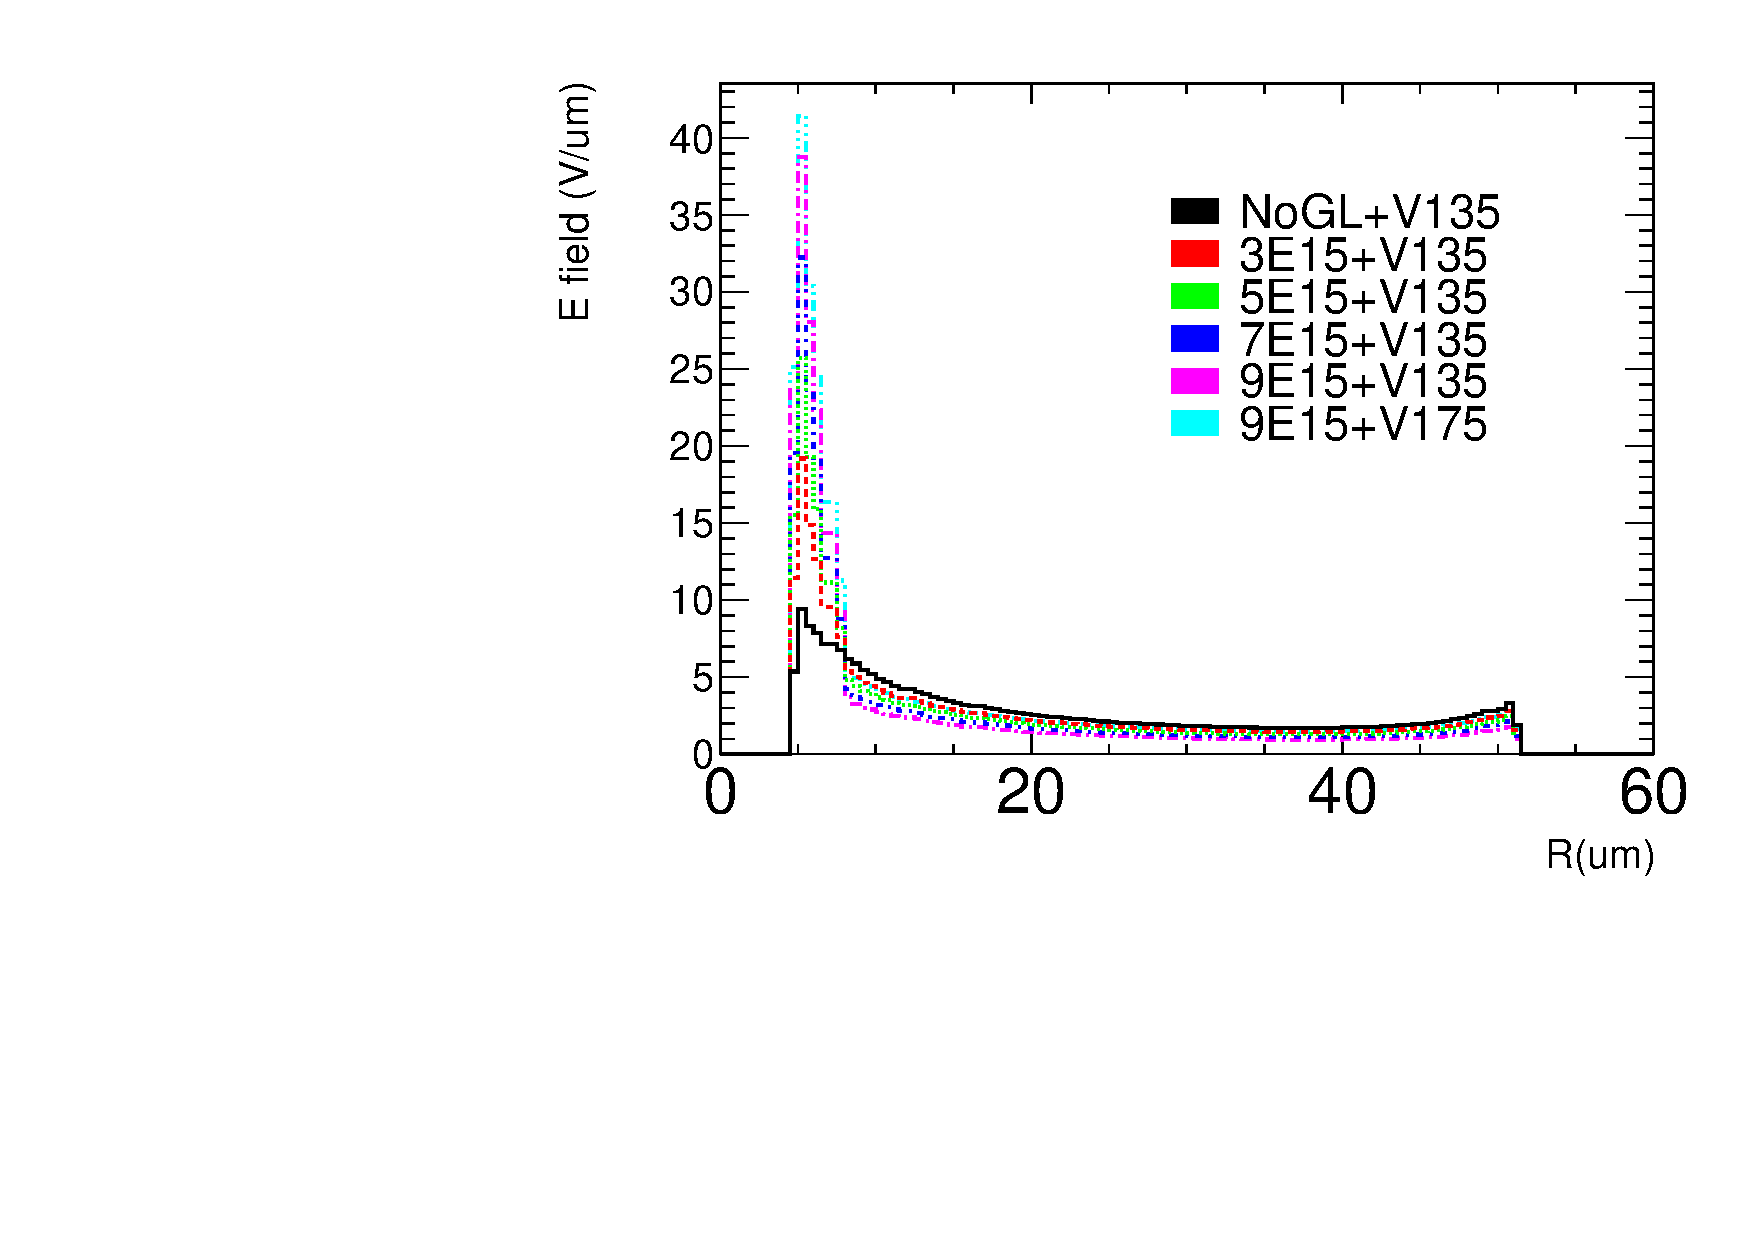
\includegraphics[width=0.35\textheight,keepaspectratio]{figures/Electric_field_IBLGAD5E_summary.pdf}
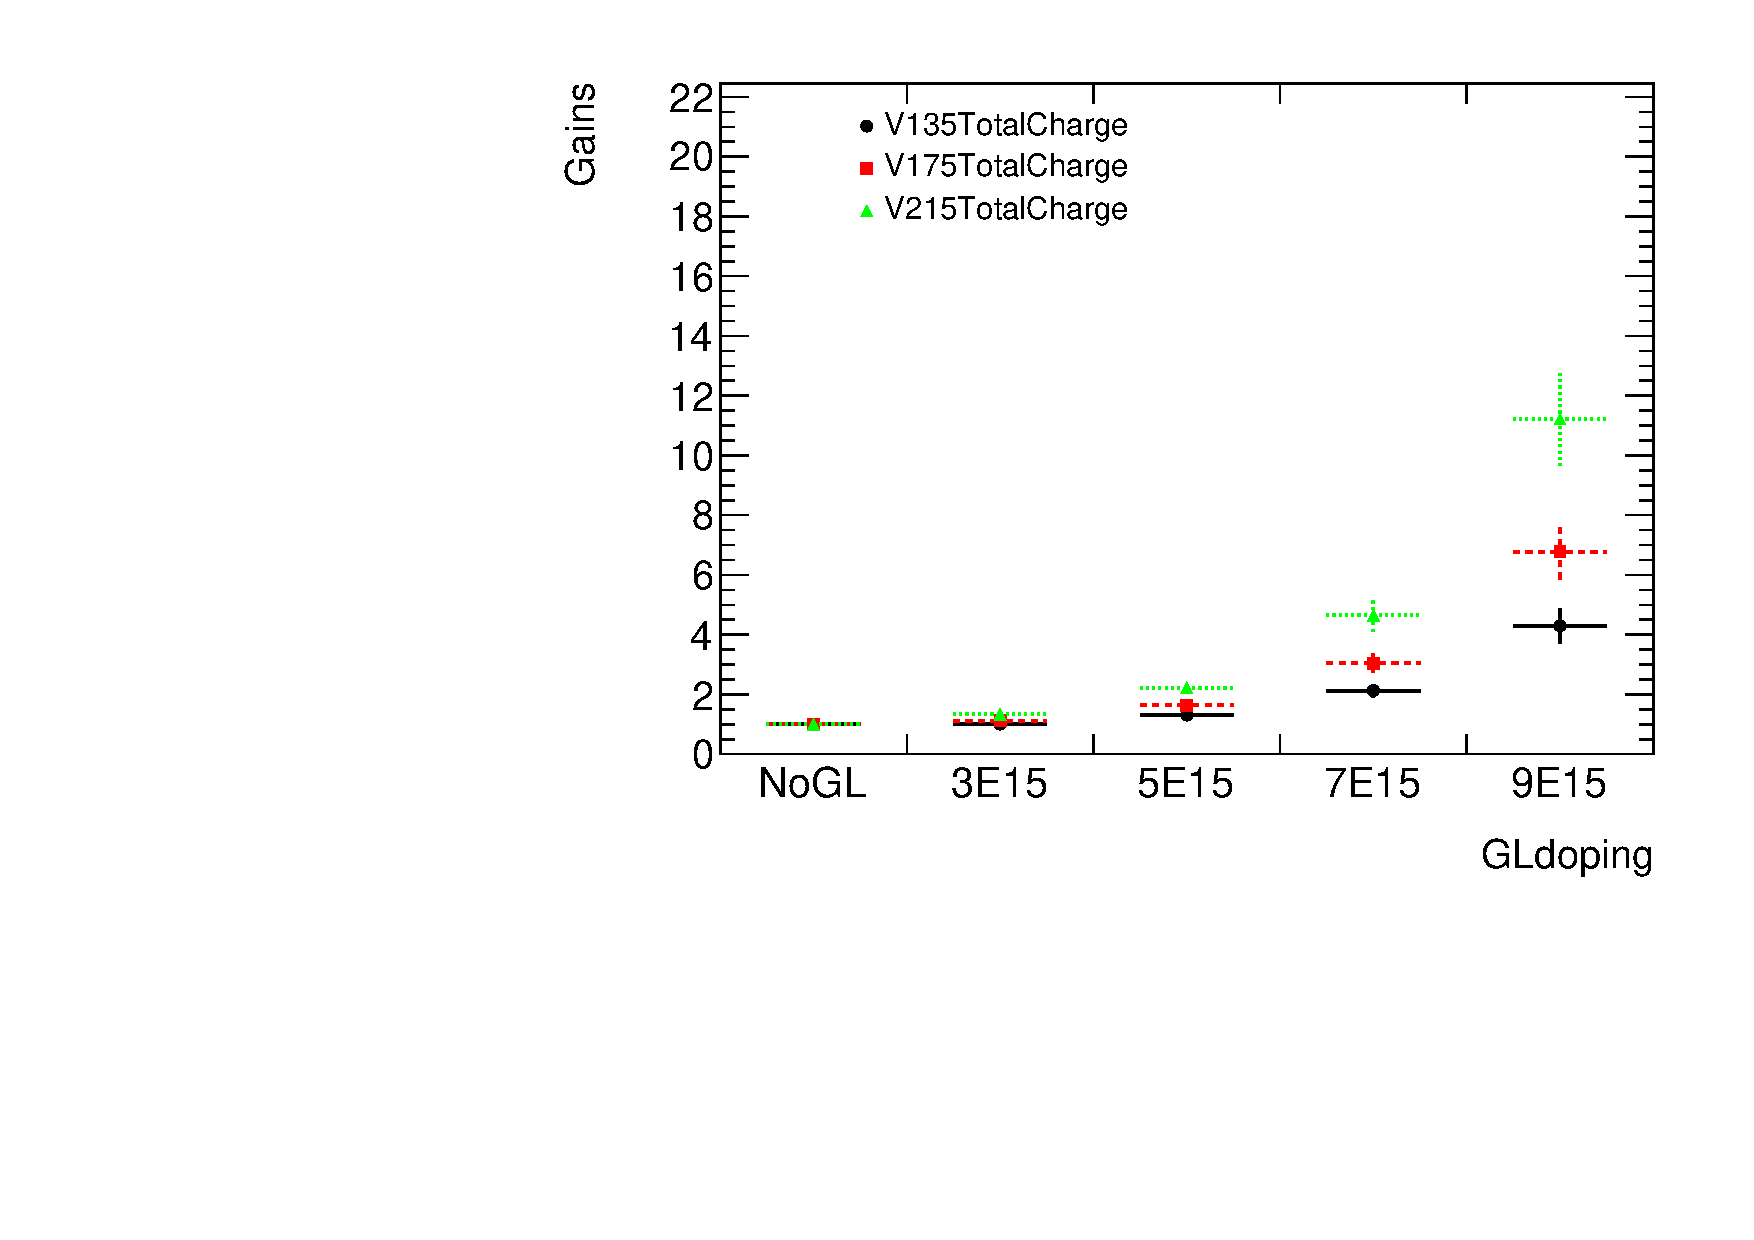
\includegraphics[width=0.35\textheight,keepaspectratio]{figures/Anatiming_timing3DIBLGAD5E_Plots_TotalChargeGLdoping.pdf}
\caption{The projection of the electric fields along the diagonal line between n+ and p+ electrodes (left) and 
the average charge collection gains for a MIP (right) as a function of GL doping densities and the bias voltages.~\label{fig:kdetgain}}
\end{center}
\end{figure}

\begin{figure}[hbtp]
\begin{center}
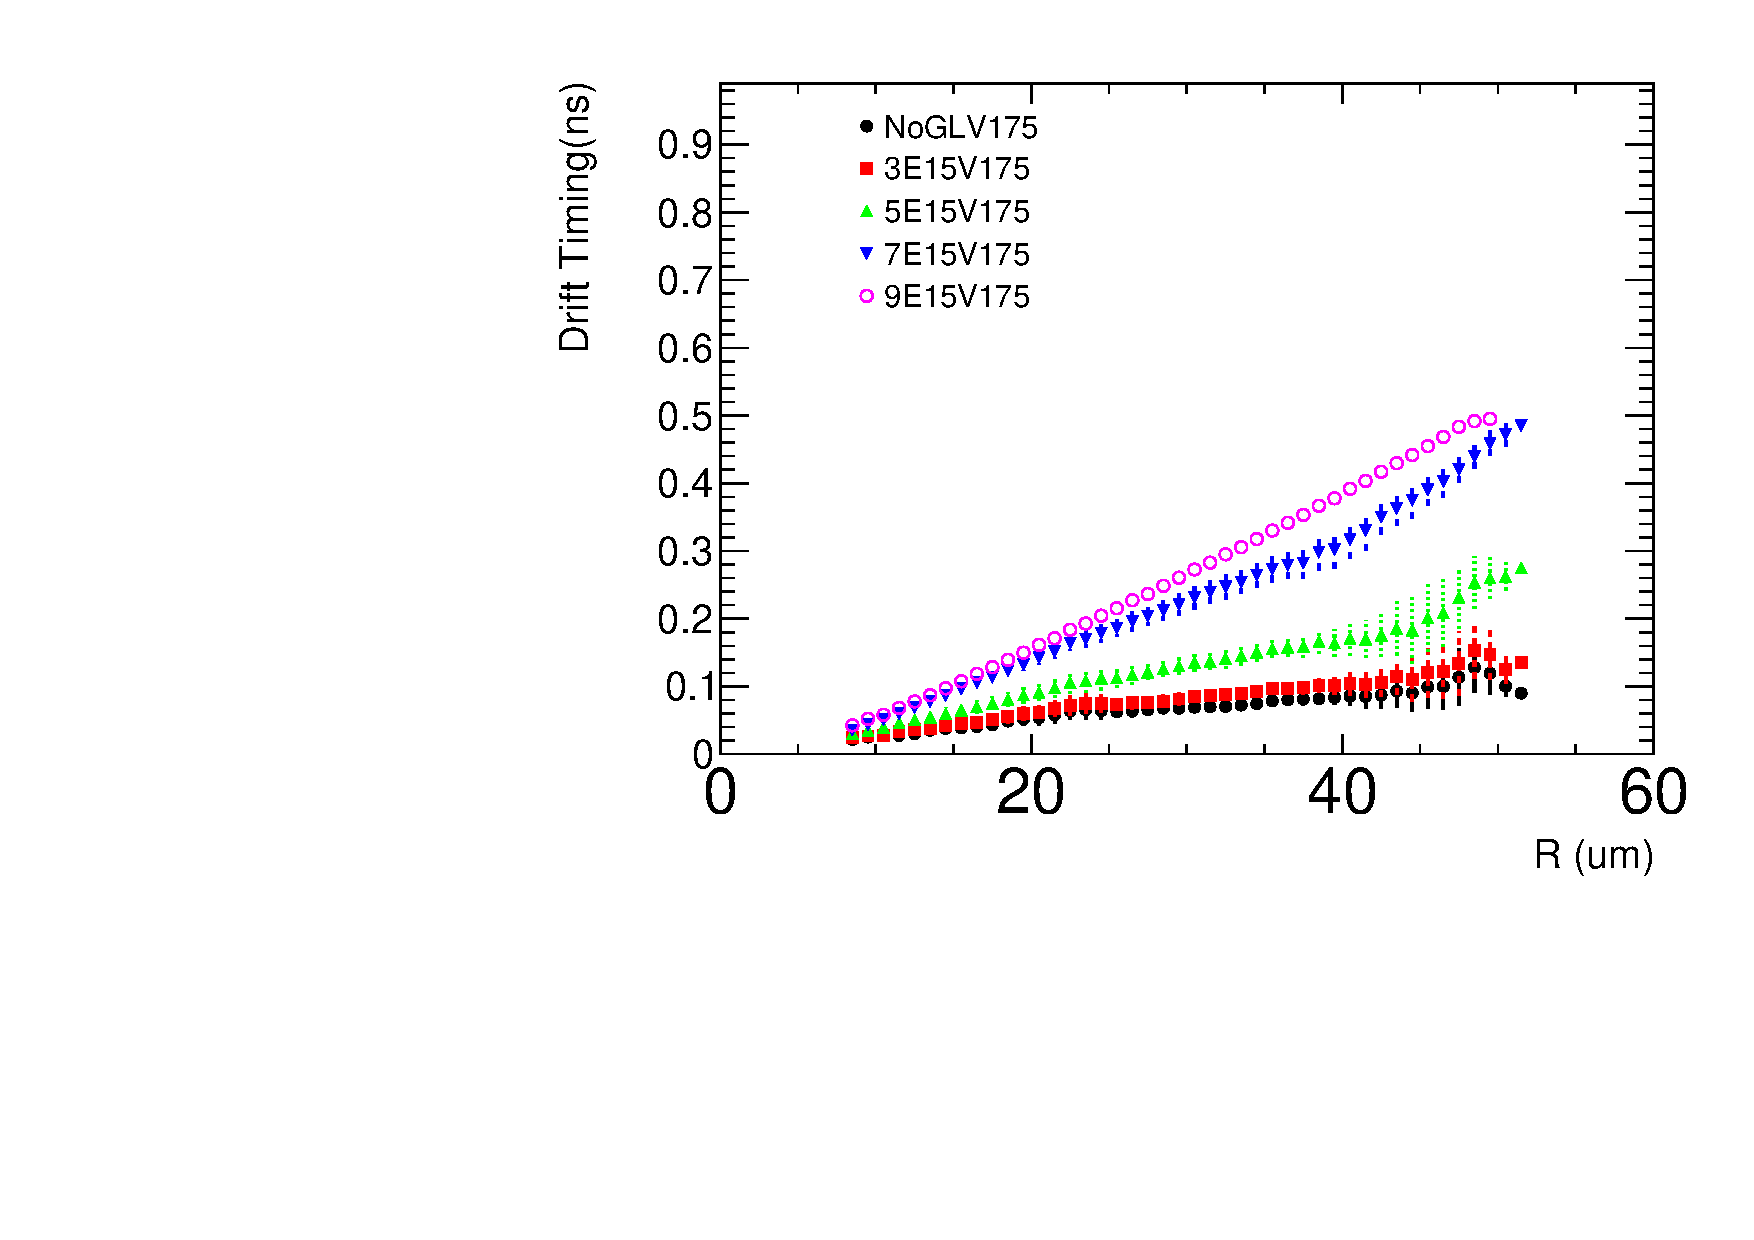
\includegraphics[width=0.25\textheight,keepaspectratio]{figures/Anatiming_timing3DIBLGAD5E_Plots_V175.pdf}
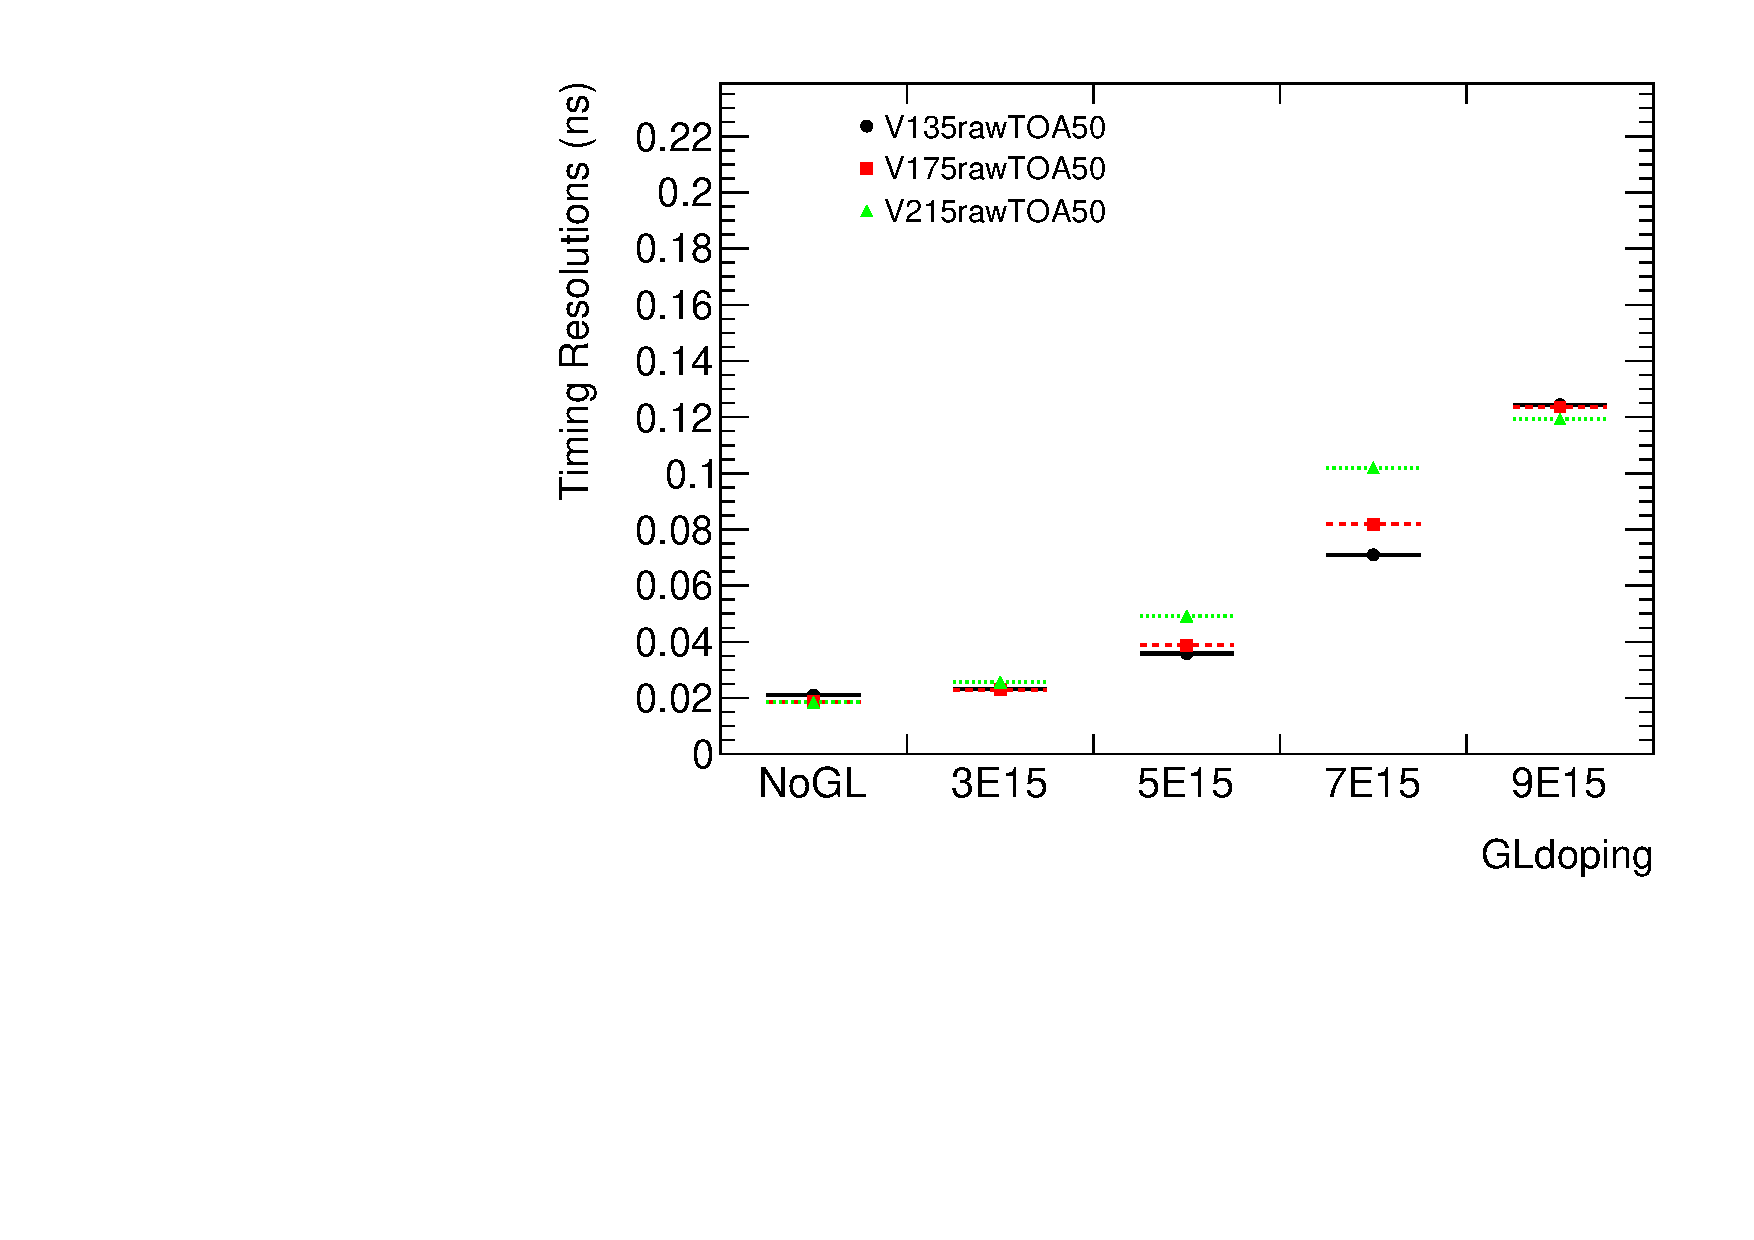
\includegraphics[width=0.25\textheight,keepaspectratio]{figures/Anatiming_timing3DIBLGAD5E_Plots_rawTOA50GLdoping.pdf}
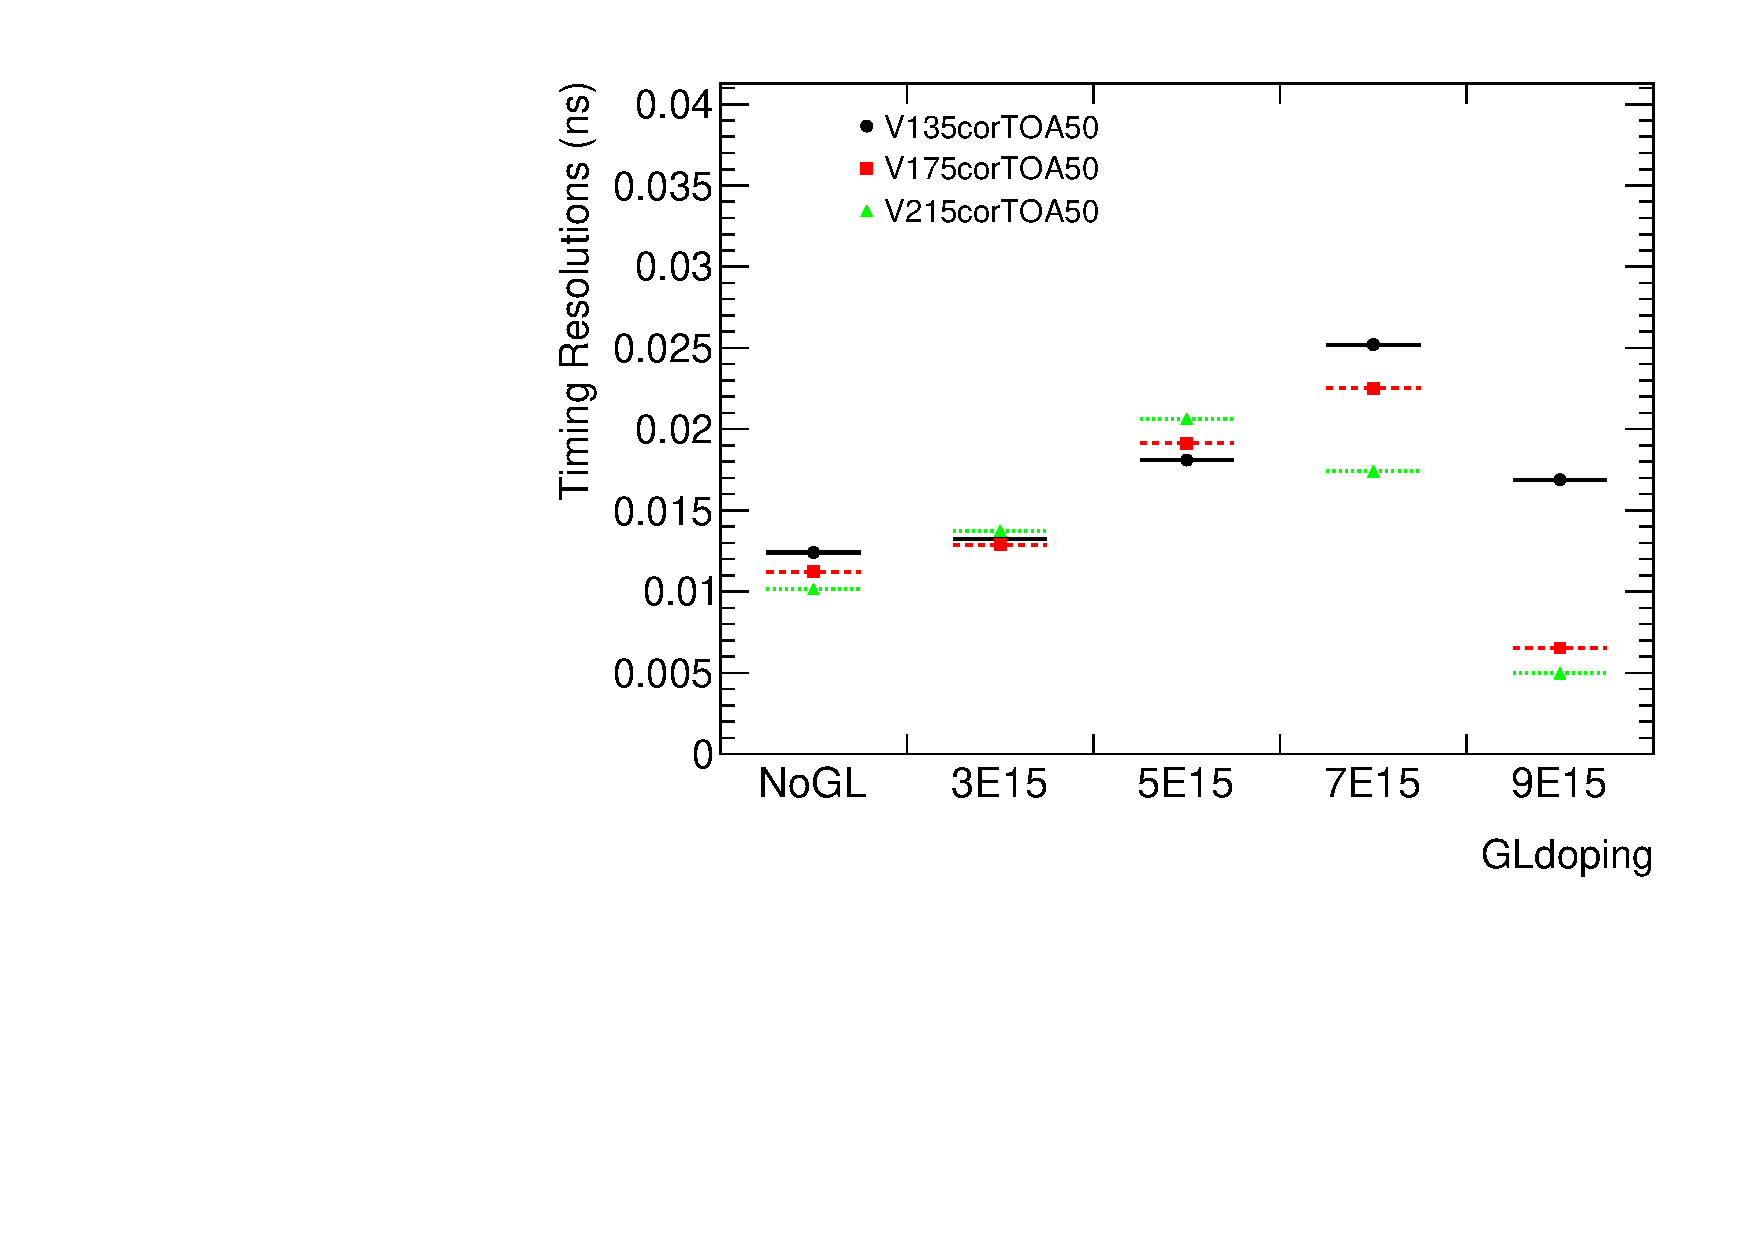
\includegraphics[width=0.25\textheight,keepaspectratio]{figures/Anatiming_timing3DIBLGAD5E_Plots_corTOA50GLdoping.pdf}
\caption{The drift-time (TOA50) as a function of drift distance from the n+ electrode (left); the average TOA50 before (middle) and 
after (right) the drift-time corrections.~\label{fig:kdettoa}}
\end{center}
\end{figure}

\section{Challengs} 

The 3D-LGAD sensor could be difficult to
produce in large-scale due to the challenges of properly doping the electrodes.
The electrodes are normally made by depositing the poly-silicon inside the holes and
they are doped by diffusion from solid or liquid source.
An alternative procedure is required to dope the gain layer properly. 

There are also significant challenges to develop the next generation of readout ASIC chips with
a pixel size of 50x50 $\mu m^2$ and a timing resolution of $\approx$~30~ps.
The current RD53 chip has a correct pixel size, but it has no proper
timing resolution. On the other hand, the ALTIROC chip designed for HGTD at ATLAS has
a timing resolution of 20~ps, but its pixel size is 1.3~mm x 1.3~mm,
too large for precision tracking~\cite{delaTaille:2018qap}.

\section{Conclusion}

In this study, we present some preliminary results on the 3D-LGAD sensor based TCAD simulation, which
could improve the signal-to-noise ratio to achieve a better timing resolution.
We aim to develop a truly 4-D silicon pixel detector with 3D sensor with both a spatial
resolution of $\approx 10~\mu m$ and a timing resolution of $\approx$30~ps
that  will open a new era for precision tracking, reducing pile-up
events and particle identification for the future colliding experiment.

\section*{Acknowledgments}

We would like to thank X.  This work was supported by the U.S.~Department of Energy, Office of Science under contract DE-AC02-05CH11231. 

\bibliographystyle{elsarticle-num}
\def\bibname{\Large\bf References}
\def\refname{\Large\bf References}
\pagestyle{plain}
\bibliography{IBL3DLGAD_NIM}

\end{document}
